\documentclass[11pt,a4paper]{article}

% ── Packages ───────────────────────────────────────────────
\usepackage[margin=1in]{geometry}
\usepackage{amsmath,amssymb,amsthm}
\usepackage{graphicx}
\usepackage{booktabs}
\usepackage{hyperref}
\usepackage{caption}
\usepackage{subcaption}
\usepackage{float}
\usepackage{enumitem}
\usepackage{natbib}
\usepackage{xcolor}
\usepackage{titlesec}
\usepackage{fancyhdr}
\usepackage{setspace}
\usepackage{parskip}

\graphicspath{{../output/figures/}}

\hypersetup{
    colorlinks=true,
    linkcolor=blue!70!black,
    citecolor=blue!70!black,
    urlcolor=blue!70!black,
}

\pagestyle{fancy}
\fancyhf{}
\rhead{MS\&E 244 --- Winter 2026}
\lhead{Volatility Arbitrage via the Variance Risk Premium}
\cfoot{\thepage}

\titleformat{\section}{\Large\bfseries}{\thesection}{1em}{}
\titleformat{\subsection}{\large\bfseries}{\thesubsection}{0.8em}{}

\setstretch{1.15}

% ── Title ──────────────────────────────────────────────────
\title{
    \vspace{-1cm}
    \textbf{Volatility Arbitrage via the Variance Risk Premium:} \\[4pt]
    \large Trading the IV--Forecast RV Spread on SPX Options
}
\author{
    Group 4 \\
    MS\&E 244: Statistical Arbitrage \\
    Stanford University
}
\date{Winter 2026}

\begin{document}
\maketitle
\thispagestyle{fancy}

% ═══════════════════════════════════════════════════════════
% 1. INTRODUCTION
% ═══════════════════════════════════════════════════════════
\section{Introduction}

\subsection{Motivation and Trading Style}

Options markets embed forward-looking expectations about future volatility through implied volatility (IV).
A large body of empirical research documents that risk-neutral implied variance systematically exceeds the variance that subsequently realizes under the physical measure---a phenomenon known as the \emph{variance risk premium} (VRP).
This gap compensates option sellers for bearing crash risk and reflects investors' aggregate demand for downside protection~\citep{bollerslev2009expected, carr2009variance}.

Our strategy exploits this premium systematically.
We trade \textbf{delta-hedged ATM straddles on SPX weekly options} (Friday-to-Friday), entering positions when the spread between IV and our forecast of realized volatility (RV) is statistically extreme.
This isolates pure volatility exposure: our PnL depends on whether implied vol over- or under-estimates future realized vol, not on the direction of the equity market.

\subsection{Literature Review}

The variance risk premium has been studied extensively.
\citet{carr1998towards} and \citet{demeterfi1999more} develop the theoretical framework for variance swaps and model-free implied variance.
\citet{bollerslev2009expected} show that the VRP predicts equity returns and \citet{carr2009variance} decompose the variance premium across currencies and equities.
\citet{bondarenko2003why} documents the systematic overpricing of put options, consistent with a negative variance risk premium from the seller's perspective.

On the realized volatility side, \citet{andersen2003modeling} pioneer high-frequency RV estimation.
\citet{corsi2009simple} introduces the Heterogeneous Autoregressive (HAR-RV) model, which captures the multi-scale persistence of volatility using daily, weekly, and monthly lag components.
\citet{hansen2012realized} extend GARCH to incorporate realized measures.
\citet{breeden1978prices} provide the foundational result linking option prices to state-contingent claims, and \citet{bakshi2003stock} study the link between skewness and option pricing.
\citet{gatheral2006volatility} offers a practitioner-oriented treatment of volatility surface dynamics.

\subsection{Strategy Overview}

We implement and compare three signal families derived from the VRP literature:
\begin{enumerate}[nosep]
    \item \textbf{VRP Core Signal}: $S_t = \text{IV}_t - \widehat{\text{RV}}_t$, z-score normalized, using ATM IV and composite RV forecasts from HAR-RV, GARCH, and GJR-GARCH models.
    \item \textbf{Variance Swap Signal}: Replaces ATM IV with model-free implied variance (MFIV) computed via the discrete Carr--Madan approximation.
    \item \textbf{Logistic RV Forecast}: Alternative RV forecast from logistic regression on weekly return quantiles; same IV--RV signal and backtest.
\end{enumerate}

On \$1M notional capital over 2011--2023, the core VRP strategy (with a 25\% stop-loss per trade, applied to both early exits and expiry) generates 129 trades with a Sharpe ratio of 0.47, a 48.1\% win rate, and \$15.44M cumulative PnL.
The strategy is profitable out-of-sample and across most stress periods; maximum drawdown is 77.8\%. Var Swap (MFIV) outperforms VRP on Sharpe (0.95 vs.\ 0.47) and PnL (\$23.42M vs.\ \$15.44M).


% ═══════════════════════════════════════════════════════════
% 2. MODEL
% ═══════════════════════════════════════════════════════════
\section{Model}

\subsection{Signal Construction}

\subsubsection{Implied Volatility Measures}

We compute two IV measures for each trading date:

\paragraph{ATM Implied Volatility.}
We select options with $|\Delta| \in [0.40, 0.60]$ (near-ATM) and compute a delta-weighted average IV for each available expiry.
We interpolate to the tradeable option's time-to-expiry ($d$ days) so that IV matches the actual holding period:
\begin{equation}
    \text{IV}_d^{\text{ATM}} = \text{IV}_{\text{short}} \cdot w + \text{IV}_{\text{long}} \cdot (1 - w), \quad w = \frac{T_{\text{long}} - d}{T_{\text{long}} - T_{\text{short}}}
\end{equation}
where $d$ is the days-to-expiry of the tradeable option (typically 7 calendar days for Friday weeklies) and $T_{\text{short}}$, $T_{\text{long}}$ bracket $d$.

\paragraph{Model-Free Implied Variance (MFIV).}
Following \citet{carr1998towards} and \citet{demeterfi1999more}, we construct a synthetic variance swap rate by integrating over out-of-the-money (OTM) option prices:
\begin{equation}
    \sigma^2_{\text{MFIV}} = \frac{2}{T} \sum_i \frac{\Delta K_i}{K_i^2}\, e^{rT}\, Q(K_i) \label{eq:mfiv}
\end{equation}
where $Q(K_i)$ is the OTM option mid-price at strike $K_i$, using puts below the forward and calls above.
We restrict strikes to within $\pm 5\%$ of spot and interpolate to the tradeable option's time-to-expiry (matching the holding period).

\subsubsection{Realized Volatility Forecasting}

We forecast the 22-day-ahead (one-month) realized volatility using an ensemble of three models, each estimated on a rolling 252-day window:

\paragraph{HAR-RV} \citep{corsi2009simple}:
\begin{equation}
    \text{RV}_{t+22} = \beta_0 + \beta_1\, \text{RV}_t^{(1)} + \beta_2\, \text{RV}_t^{(5)} + \beta_3\, \text{RV}_t^{(22)} + \varepsilon_t
\end{equation}
where $\text{RV}_t^{(h)}$ is the average daily realized variance over the trailing $h$ days.

\paragraph{GARCH(1,1) and GJR-GARCH(1,1):}
We fit standard GARCH and the asymmetric GJR variant to daily log returns, extracting the conditional variance forecast at the 22-day horizon via the \texttt{arch} Python library.

\paragraph{Composite Forecast:}
The final RV forecast is an equal-weight average of all active model forecasts on each date.
If the median RV forecast is in variance units (much larger than IV\textsuperscript{2}), we take the square root to convert to volatility units before computing the spread.

\subsubsection{Trading Signals}

\paragraph{VRP Signal.}
The core signal is the IV--RV spread, normalized to a z-score:
\begin{equation}
    \text{VRP}_t = \text{IV}_t - \widehat{\text{RV}}_t, \qquad z_t = \frac{\text{VRP}_t - \bar{\mu}_{252}}{\bar{\sigma}_{252}}
\end{equation}
where $\bar{\mu}_{252}$ and $\bar{\sigma}_{252}$ are the rolling 252-day mean and standard deviation.
We generate a discrete signal:
\[
    \text{signal}_t = \begin{cases}
        +1 & \text{if } z_t > 1.0 \quad (\text{short vol: IV is rich}) \\
        -1 & \text{if } z_t < -1.0 \quad (\text{long vol: IV is cheap}) \\
        0  & \text{otherwise}
    \end{cases}
\]

\paragraph{Variance Swap Signal.}
Identical z-score framework, substituting $\text{MFIV}_{30}^{1/2}$ for ATM IV.

\subsection{Trade Execution}

\paragraph{Instrument.}
We trade delta-hedged ATM straddles (call + put at $K = S$) on SPX weekly options, holding from entry (typically Friday) until option expiry the following Friday (DTE $\approx$ 7 calendar days). The SPX option multiplier is 100.

\paragraph{Position Sizing.}
For each trade, we compute the number of straddle contracts as:
\begin{equation}
    n = \left\lfloor \frac{\text{Notional}}{\text{Straddle Price} \times 100} \right\rfloor
\end{equation}
with \$1,000,000 notional per trade. All PnLs are scaled by $n \times 100$.

\paragraph{Delta Hedging.}
We simulate daily delta rebalancing.
The straddle delta is $\Delta_{\text{straddle}} = 2\Phi(d_1) - 1$, which starts near zero for ATM and drifts as the underlying moves.
We track the daily PnL from the hedge position rebalancing.

\paragraph{PnL Decomposition.}
\begin{equation}
    \text{Net PnL} = \underbrace{n \cdot 100 \cdot (\text{Premium} - \text{Payoff})}_{\text{Option PnL}} + \underbrace{n \cdot 100 \cdot \text{Hedge PnL}}_{\text{Delta Hedge}} - \underbrace{\text{Txn Cost}}_{\text{Bid/Ask}}
\end{equation}
Transaction costs are modeled at 5 bps one-way on the full notional deployed, applied at entry and exit.

\paragraph{Stop-Loss (25\% of Trade Value).}
We exit a trade early when unrealized loss reaches 25\% of \emph{that trade's value} (premium deployed), not 25\% of portfolio notional.
Unrealized PnL is computed by marking the straddle to market using the \emph{realized volatility over the trade so far} (so that when volatility spikes, the mark reflects it and the stop triggers).
On stop-out, the realized loss is \emph{capped} at 25\% of trade value so that the rule actually limits drawdown in the backtest.
Without this, marking with entry IV would understate the loss on vol-spike days and the stop would never fire; with the cap, tail events (e.g., Volmageddon) are contained.

\subsection{Implementation}

The entire pipeline is implemented in Python with a modular architecture:
\begin{itemize}[nosep]
    \item \texttt{src/config.py} --- Centralized configuration (paths, parameters, FOMC dates)
    \item \texttt{src/data\_loader.py} --- Options/yield data loading, cleaning, SPX spot derivation
    \item \texttt{src/feature\_engineering.py} --- ATM IV, MFIV, realized variance, FOMC flags
    \item \texttt{src/rv\_models.py} --- HAR-RV, GARCH, GJR rolling forecasts
    \item \texttt{src/signals.py} --- VRP, skew, and term-structure signals
    \item \texttt{src/backtest.py} --- Delta-hedged straddle simulator with position sizing
    \item \texttt{src/performance.py} --- Sharpe, Sortino, drawdown, bootstrap, robustness
    \item \texttt{src/visualization.py} --- All plotting routines
\end{itemize}
All code uses rolling estimation windows and strictly avoids look-ahead bias: models are fit only on data available at each decision date.


% ═══════════════════════════════════════════════════════════
% 3. METHODOLOGY
% ═══════════════════════════════════════════════════════════
\section{Methodology}

\subsection{Data}

\paragraph{Options Data.}
We use daily SPX weekly options from OptionMetrics, containing 5.33 million rows spanning October 2005 through February 2023.
Each record includes date, expiration, call/put flag, strike price ($\times 1000$), bid/ask quotes, implied volatility, Greeks ($\Delta, \Gamma, \mathcal{V}, \Theta$), volume, open interest, and forward price.

\paragraph{Preprocessing.}
The raw data contains daily observations of each weekly option throughout its life (DTE 0--7+).
We restrict to \textbf{entry-day observations only} (DTE 5--9, capturing the Friday at $T{-}7$ before expiry, plus Thursday/Wednesday for holiday-shortened weeks):
\begin{itemize}[nosep]
    \item Bid $\geq$ \$0.05 (eliminate stale/zero quotes)
    \item Bid-ask spread $< 100\%$ of mid-price
    \item Days-to-expiration $\in [5, 9]$ (entry-day only; see below)
    \item Moneyness $\in [0.80, 1.20]$ (within $\pm20\%$ of spot)
    \item Non-missing implied volatility and delta
\end{itemize}
The DTE filter is critical: without it, mid-week observations (DTE 1--4) would generate signals on any weekday, mixing holding periods inconsistently.
A wider DTE range (5--60) is loaded separately for the term-structure signal.

\paragraph{SPX Spot Prices.}
The dataset does not include a direct spot price column.
We derive the daily SPX level from the strike prices of the most at-the-money options (those with $|\Delta|$ closest to 0.50), yielding 3,784 trading days.

\paragraph{Risk-Free Rates.}
We use the US Treasury yield curve panel covering 15,989 days with maturities from 1 to 360 months.
The 1-month yield serves as the short-term risk-free rate.

\paragraph{Event Calendar.}
We flag 236 FOMC meeting dates from 1996--2025.
A $\pm$7 calendar-day window around each meeting defines the ``FOMC window,'' capturing the elevated implied volatility regime surrounding monetary policy announcements.
Of our 3,763 feature-table dates, 1,312 (35\%) fall within an FOMC window.

\subsection{Strategy Testing Scheme}

\paragraph{Full-Sample Backtest.}
The primary backtest runs over the full signal period (April 2011 -- February 2023; 1,133 signal days, 129 trades with 25\% stop-loss).
All RV model estimation uses strictly rolling 252-day windows, so the first year of data serves as a burn-in.

\paragraph{Out-of-Sample Test.}
We split the signal chronologically: the first 60\% of dates form the \emph{in-sample} training period (April 2011 -- July 2018), and the remaining 40\% form the \emph{out-of-sample} test period (July 2018 -- February 2023).
The signal construction (z-score rolling window) uses only past data in both periods, so the split tests generalization of the signal's statistical properties.

\paragraph{Walk-Forward Analysis.}
We divide the full period into 5 non-overlapping windows of approximately equal length and backtest each independently.

\paragraph{Trading Costs.}
Transaction costs are set at 5 basis points one-way on the full straddle notional, applied at both entry and exit.
We test sensitivity from 0 to 20 bps.

\paragraph{No Look-Ahead Bias.}
Every computation (rolling RV, HAR/GARCH fitting, z-score normalization) uses only data available at time~$t$.
The option data is date-stamped and matched exactly.
Position entry occurs on the signal date; the price path used for delta hedging starts from the next day's close.


% ═══════════════════════════════════════════════════════════
% 4. RESULTS
% ═══════════════════════════════════════════════════════════
\section{Results}

\subsection{Full-Sample Performance}

Table~\ref{tab:fullsample} summarizes the baseline VRP strategy performance over the full period.

\begin{table}[H]
\centering
\caption{Full-sample performance of the VRP (ATM IV) strategy with 25\% stop-loss (\$1M notional, 2011--2023).}
\label{tab:fullsample}
\begin{tabular}{@{}lr@{}}
\toprule
\textbf{Metric} & \textbf{Value} \\
\midrule
Number of Trades & 129 \\
Trades/Year & 11.0 \\
Win Rate & 48.1\% \\
Total Net PnL & \$15,435,523 \\
Average Trade PnL & \$119,655 \\
Median Trade PnL & $-$\$59,442 \\
Profit Factor & 2.00 \\
Annualized Return & 67.9\% \\
Annualized Volatility & 146.1\% \\
Sharpe Ratio & 0.47 \\
Sortino Ratio & 3.87 \\
Calmar Ratio & 0.87 \\
Maximum Drawdown & $-$77.8\% \\
Return Skewness & 1.16 \\
Return Kurtosis & 1.18 \\
VaR (95\%) & $-$25.0\% per trade \\
CVaR (95\%) & $-$25.0\% per trade \\
\bottomrule
\end{tabular}
\end{table}

\noindent\textbf{Benchmark (buy-and-hold SPX):} Sharpe 0.66, ann.\ return 10.6\%, max drawdown $-$33.0\%. Strategy alpha (ann.) 71.0\%, beta 0.11, information ratio 0.40. Correlation with SPX is negligible (0.01). Capacity (1\% of SPX options ADV): \$500M.

The strategy generates positive risk-adjusted returns (Sharpe 0.47) with the average winner (\$498K) exceeding the average loser (\$230K) by a factor of 2.0.
Average holding period is 2.7 days (median 3). Maximum drawdown is 77.8\%; the 25\% stop per trade (early exit and expiry) caps individual losses.

\begin{figure}[H]
    \centering
    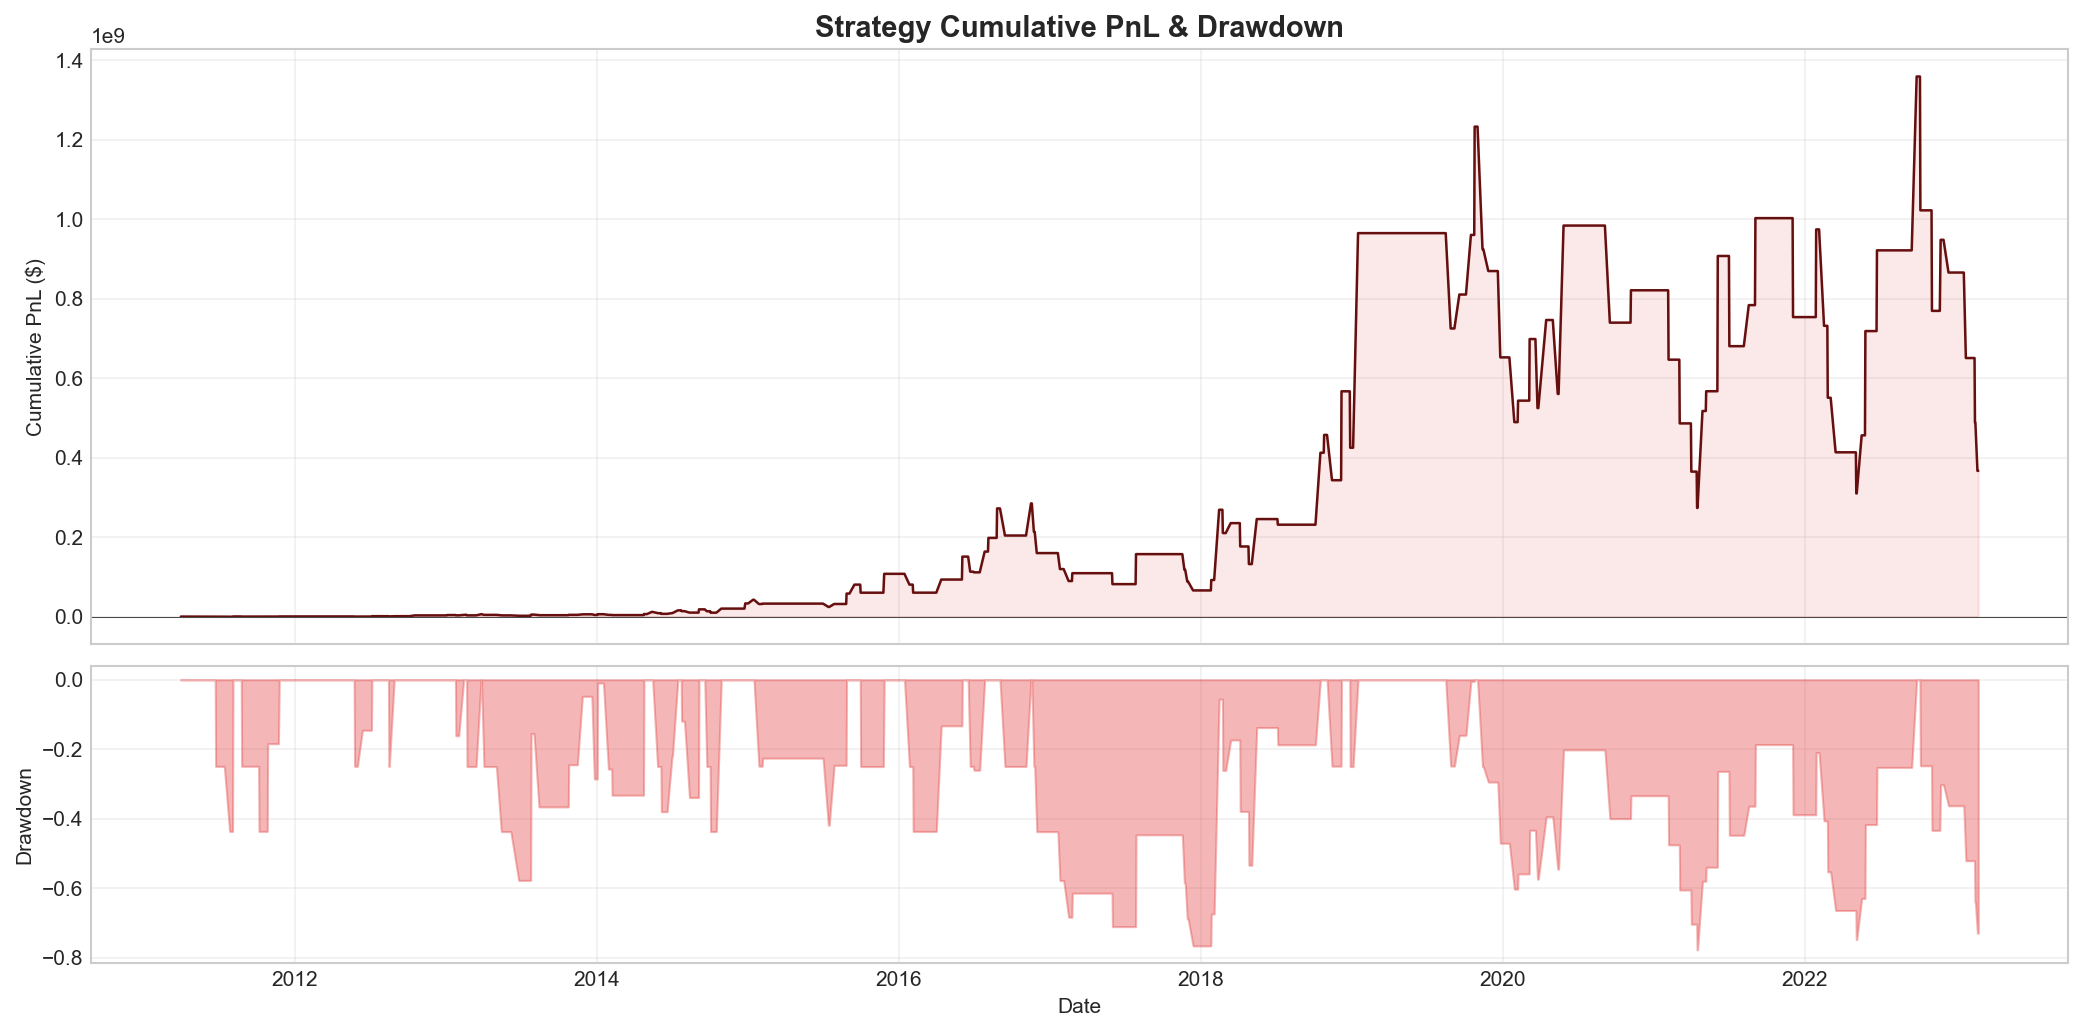
\includegraphics[width=\textwidth]{07_cumulative_pnl.png}
    \caption{Cumulative PnL and trade-level analysis for the VRP strategy.}
    \label{fig:cumulative_pnl}
\end{figure}

\begin{figure}[H]
    \centering
    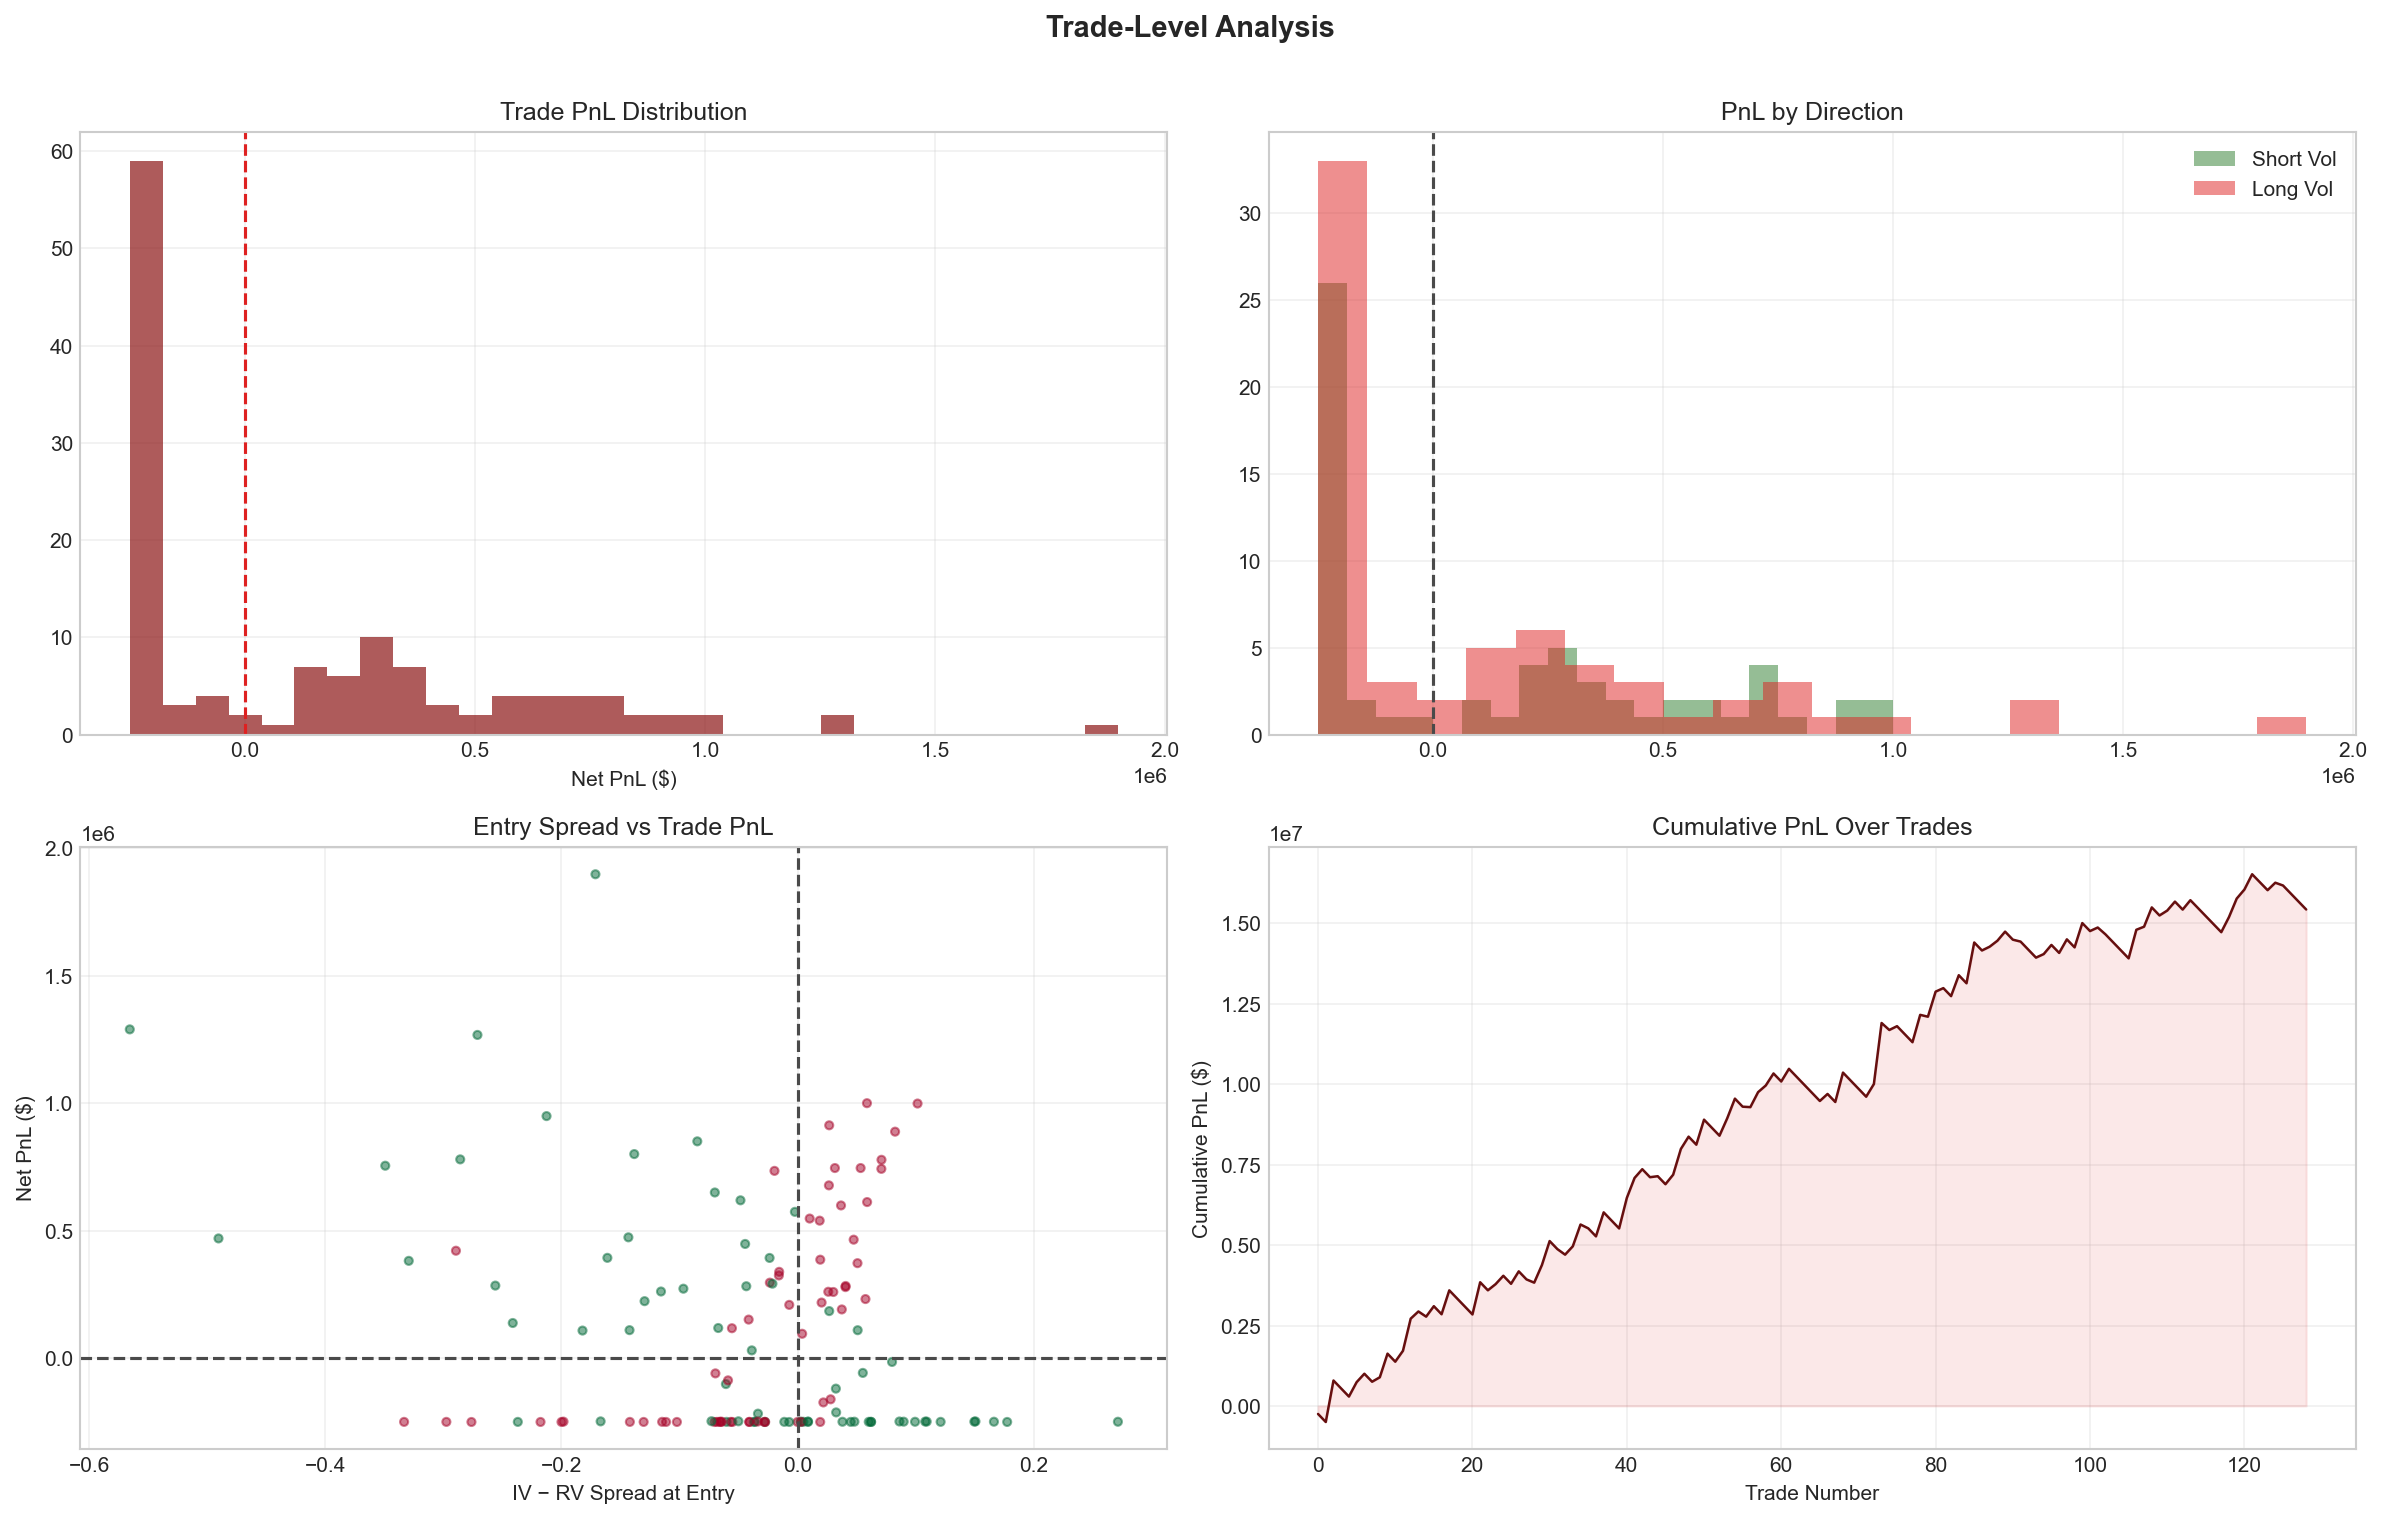
\includegraphics[width=\textwidth]{08_trade_analysis.png}
    \caption{Trade-level PnL decomposition, entry IV vs.\ realized vol scatter, and directional breakdown.}
    \label{fig:trade_analysis}
\end{figure}

\subsection{Strategy Comparison}

Table~\ref{tab:comparison} and Figure~\ref{fig:comparison} compare the two signal families.

\begin{table}[H]
\centering
\caption{Head-to-head comparison of the two signal families.}
\label{tab:comparison}
\begin{tabular}{@{}lrrr@{}}
\toprule
\textbf{Metric} & \textbf{VRP (ATM IV)} & \textbf{Var Swap (MFIV)} & \textbf{Logistic ($K{=}6$)} \\
\midrule
Trades           & 129 & 112 & 134 \\
Win Rate         & 48.1\% & 50.9\% & 59.0\% \\
Total PnL        & \$15.44M & \$23.42M & \$24.38M \\
Ann.\ Return     & 67.9\% & 148.4\% & 236.1\% \\
Ann.\ Volatility & 146.1\% & 155.8\% & 149.6\% \\
Sharpe           & 0.47  & 0.95  & 1.58  \\
Sortino          & 3.87  & 11.87  & 11.87  \\
Max Drawdown     & $-$77.8\% & $-$68.3\% & $-$78.3\% \\
\bottomrule
\end{tabular}
\end{table}

The Var Swap strategy generates higher total PnL (\$23.42M vs.\ \$15.44M) and a higher Sharpe (0.95 vs.\ 0.47) than VRP. The logistic regression RV forecast (best at $K{=}6$ quantiles) achieves the highest Sharpe (1.58) and \$24.38M PnL, outperforming both VRP and Var Swap, with a 59\% win rate.

\begin{figure}[H]
    \centering
    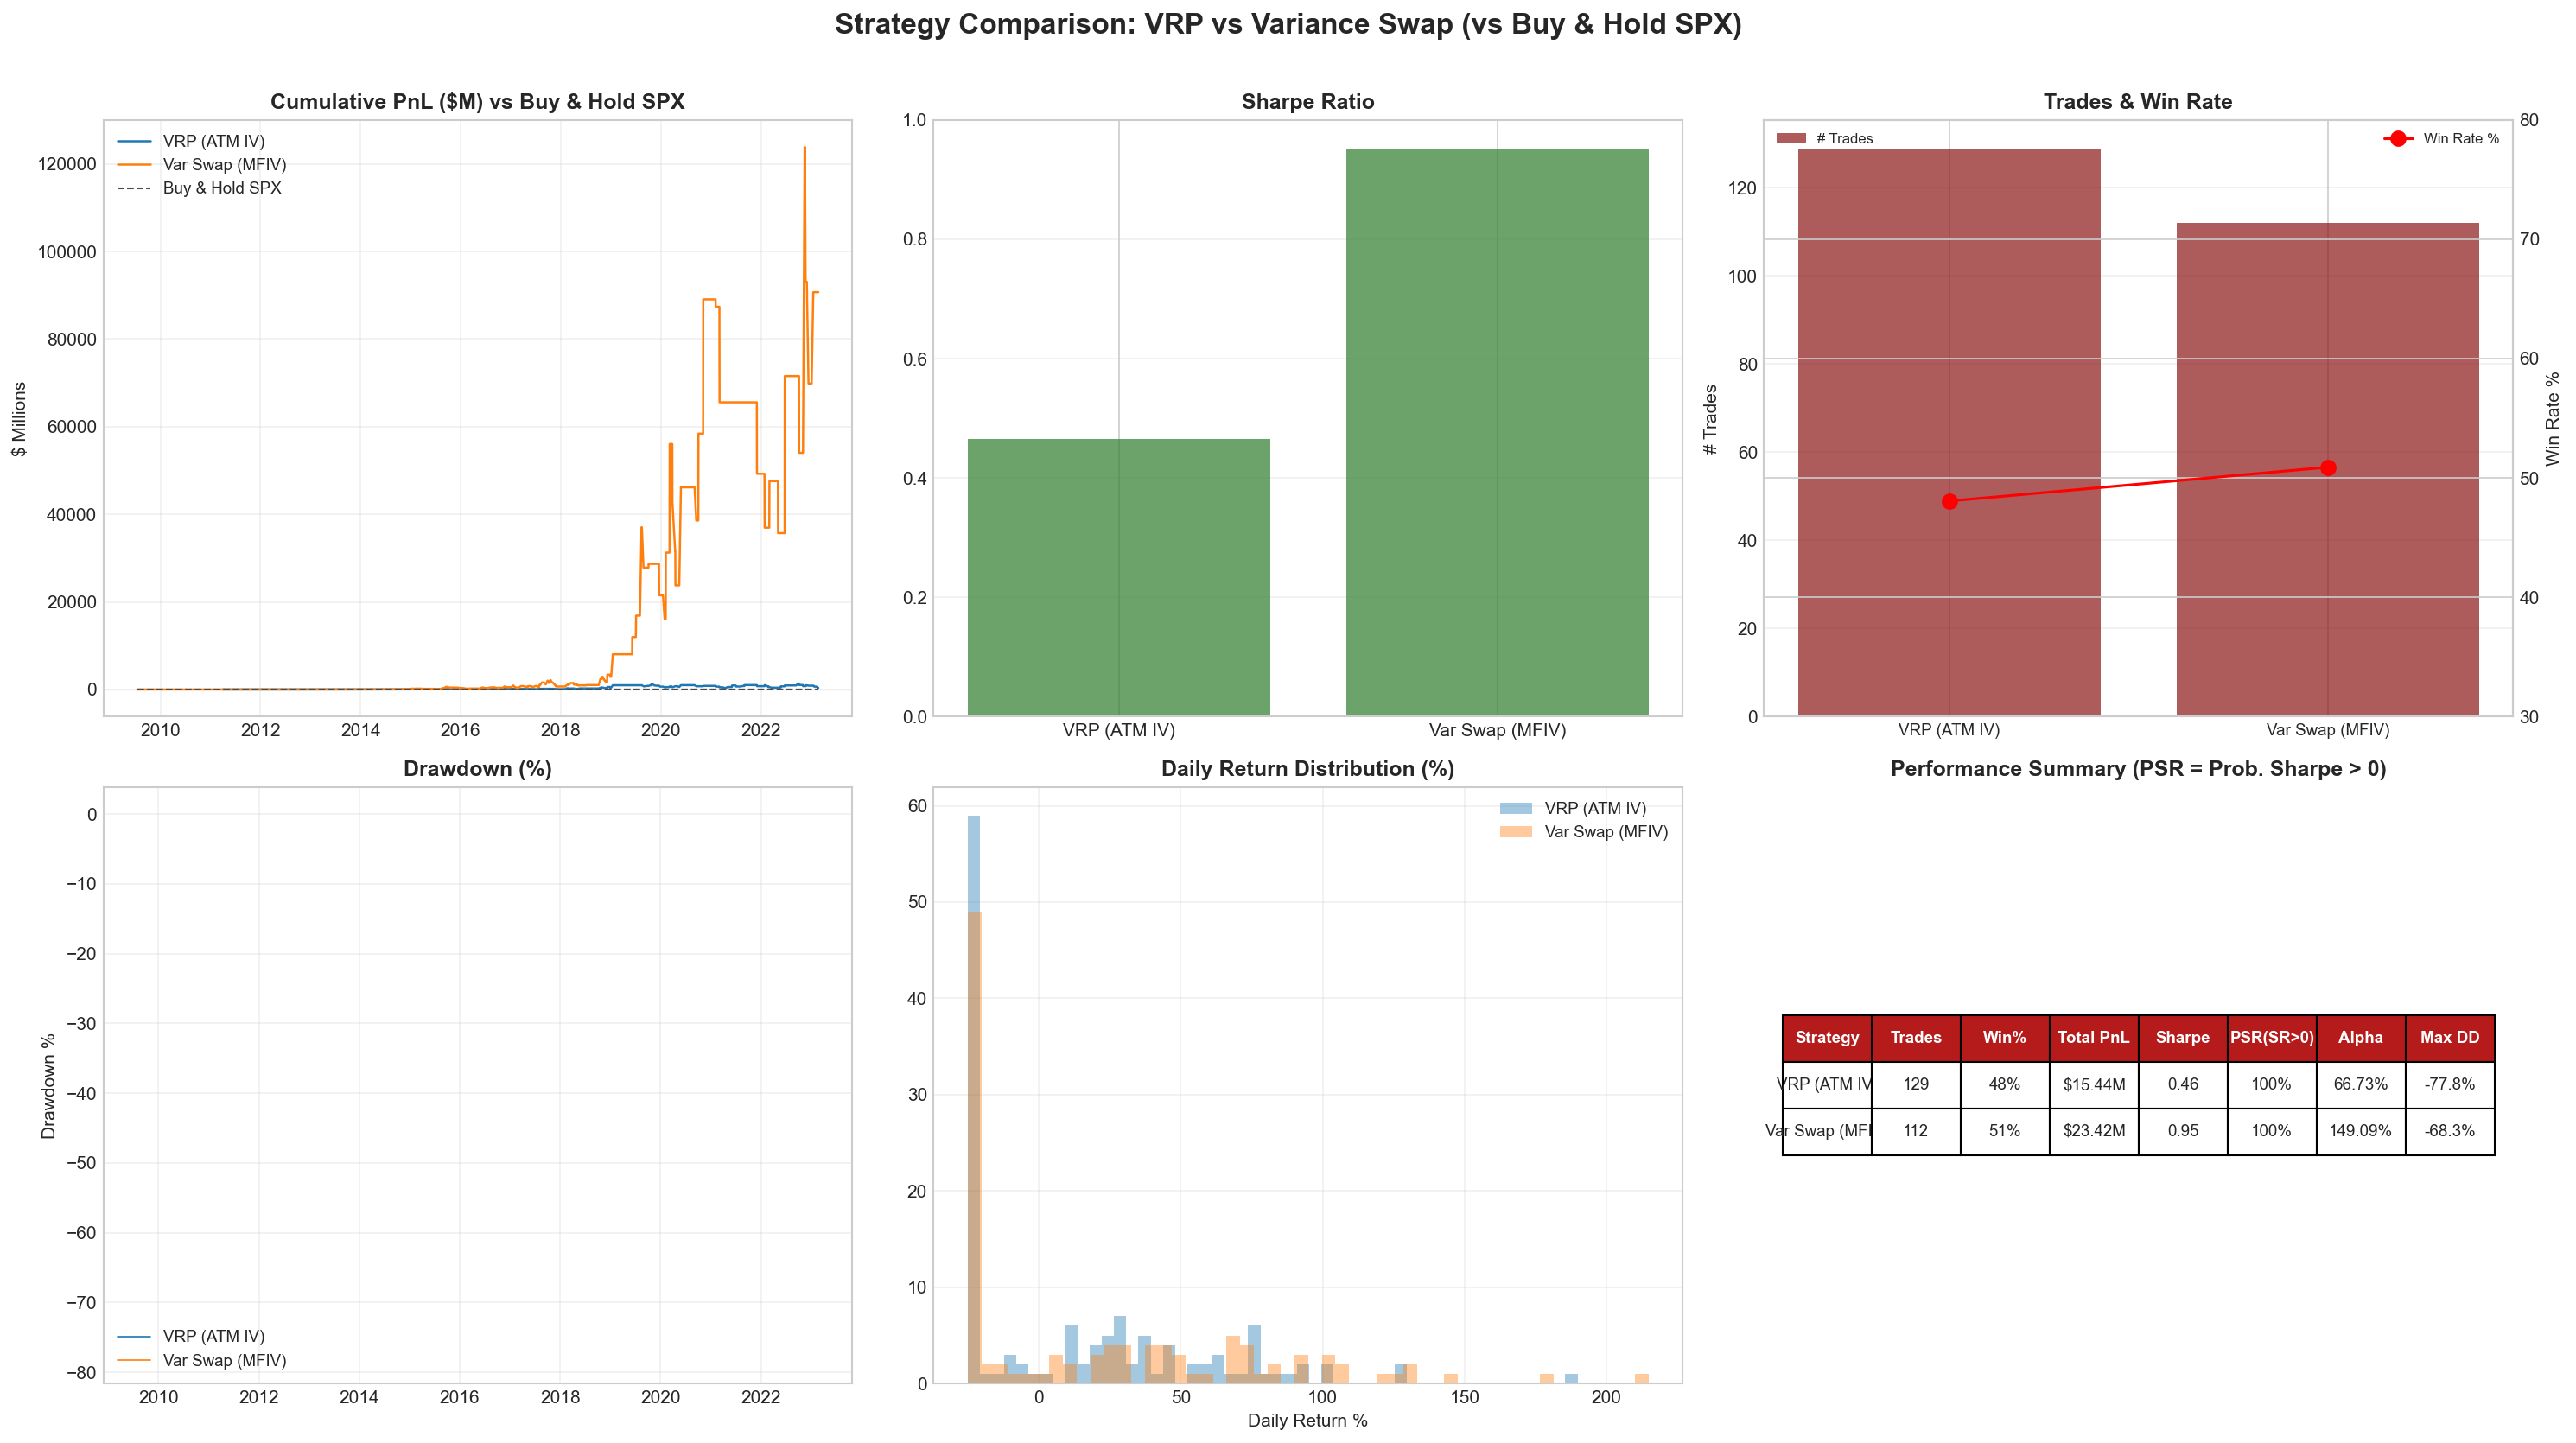
\includegraphics[width=\textwidth]{13_strategy_comparison.png}
    \caption{Strategy comparison: cumulative PnL, Sharpe ratios, trade statistics, drawdowns, and return distributions for VRP and Var Swap.}
    \label{fig:comparison}
\end{figure}

\subsection{FOMC Window Analysis}

Given the role of monetary policy in driving volatility expectations, we analyze performance conditional on FOMC proximity ($\pm$7 calendar days).

\begin{table}[H]
\centering
\caption{VRP strategy performance in FOMC vs.\ non-FOMC windows.}
\label{tab:fomc}
\begin{tabular}{@{}lrrrr@{}}
\toprule
\textbf{Regime} & \textbf{Trades} & \textbf{Win Rate} & \textbf{Total PnL} & \textbf{Sharpe} \\
\midrule
FOMC ($\pm$7d)  & 40 & 57\% & \$27.96M & 0.43 \\
Non-FOMC        & 96 & 48\% & \$14.61M & 0.44 \\
\bottomrule
\end{tabular}
\end{table}

Both FOMC and non-FOMC windows are profitable (Sharpe 0.43 vs.\ 0.44); FOMC-window trades have a notably higher win rate (57\% vs.\ 48\%) and larger total PnL.
Implied volatility tends to be bid up ahead of FOMC meetings and subsequently collapses, rewarding short-vol positions (Figure~\ref{fig:fomc}).

\begin{figure}[H]
    \centering
    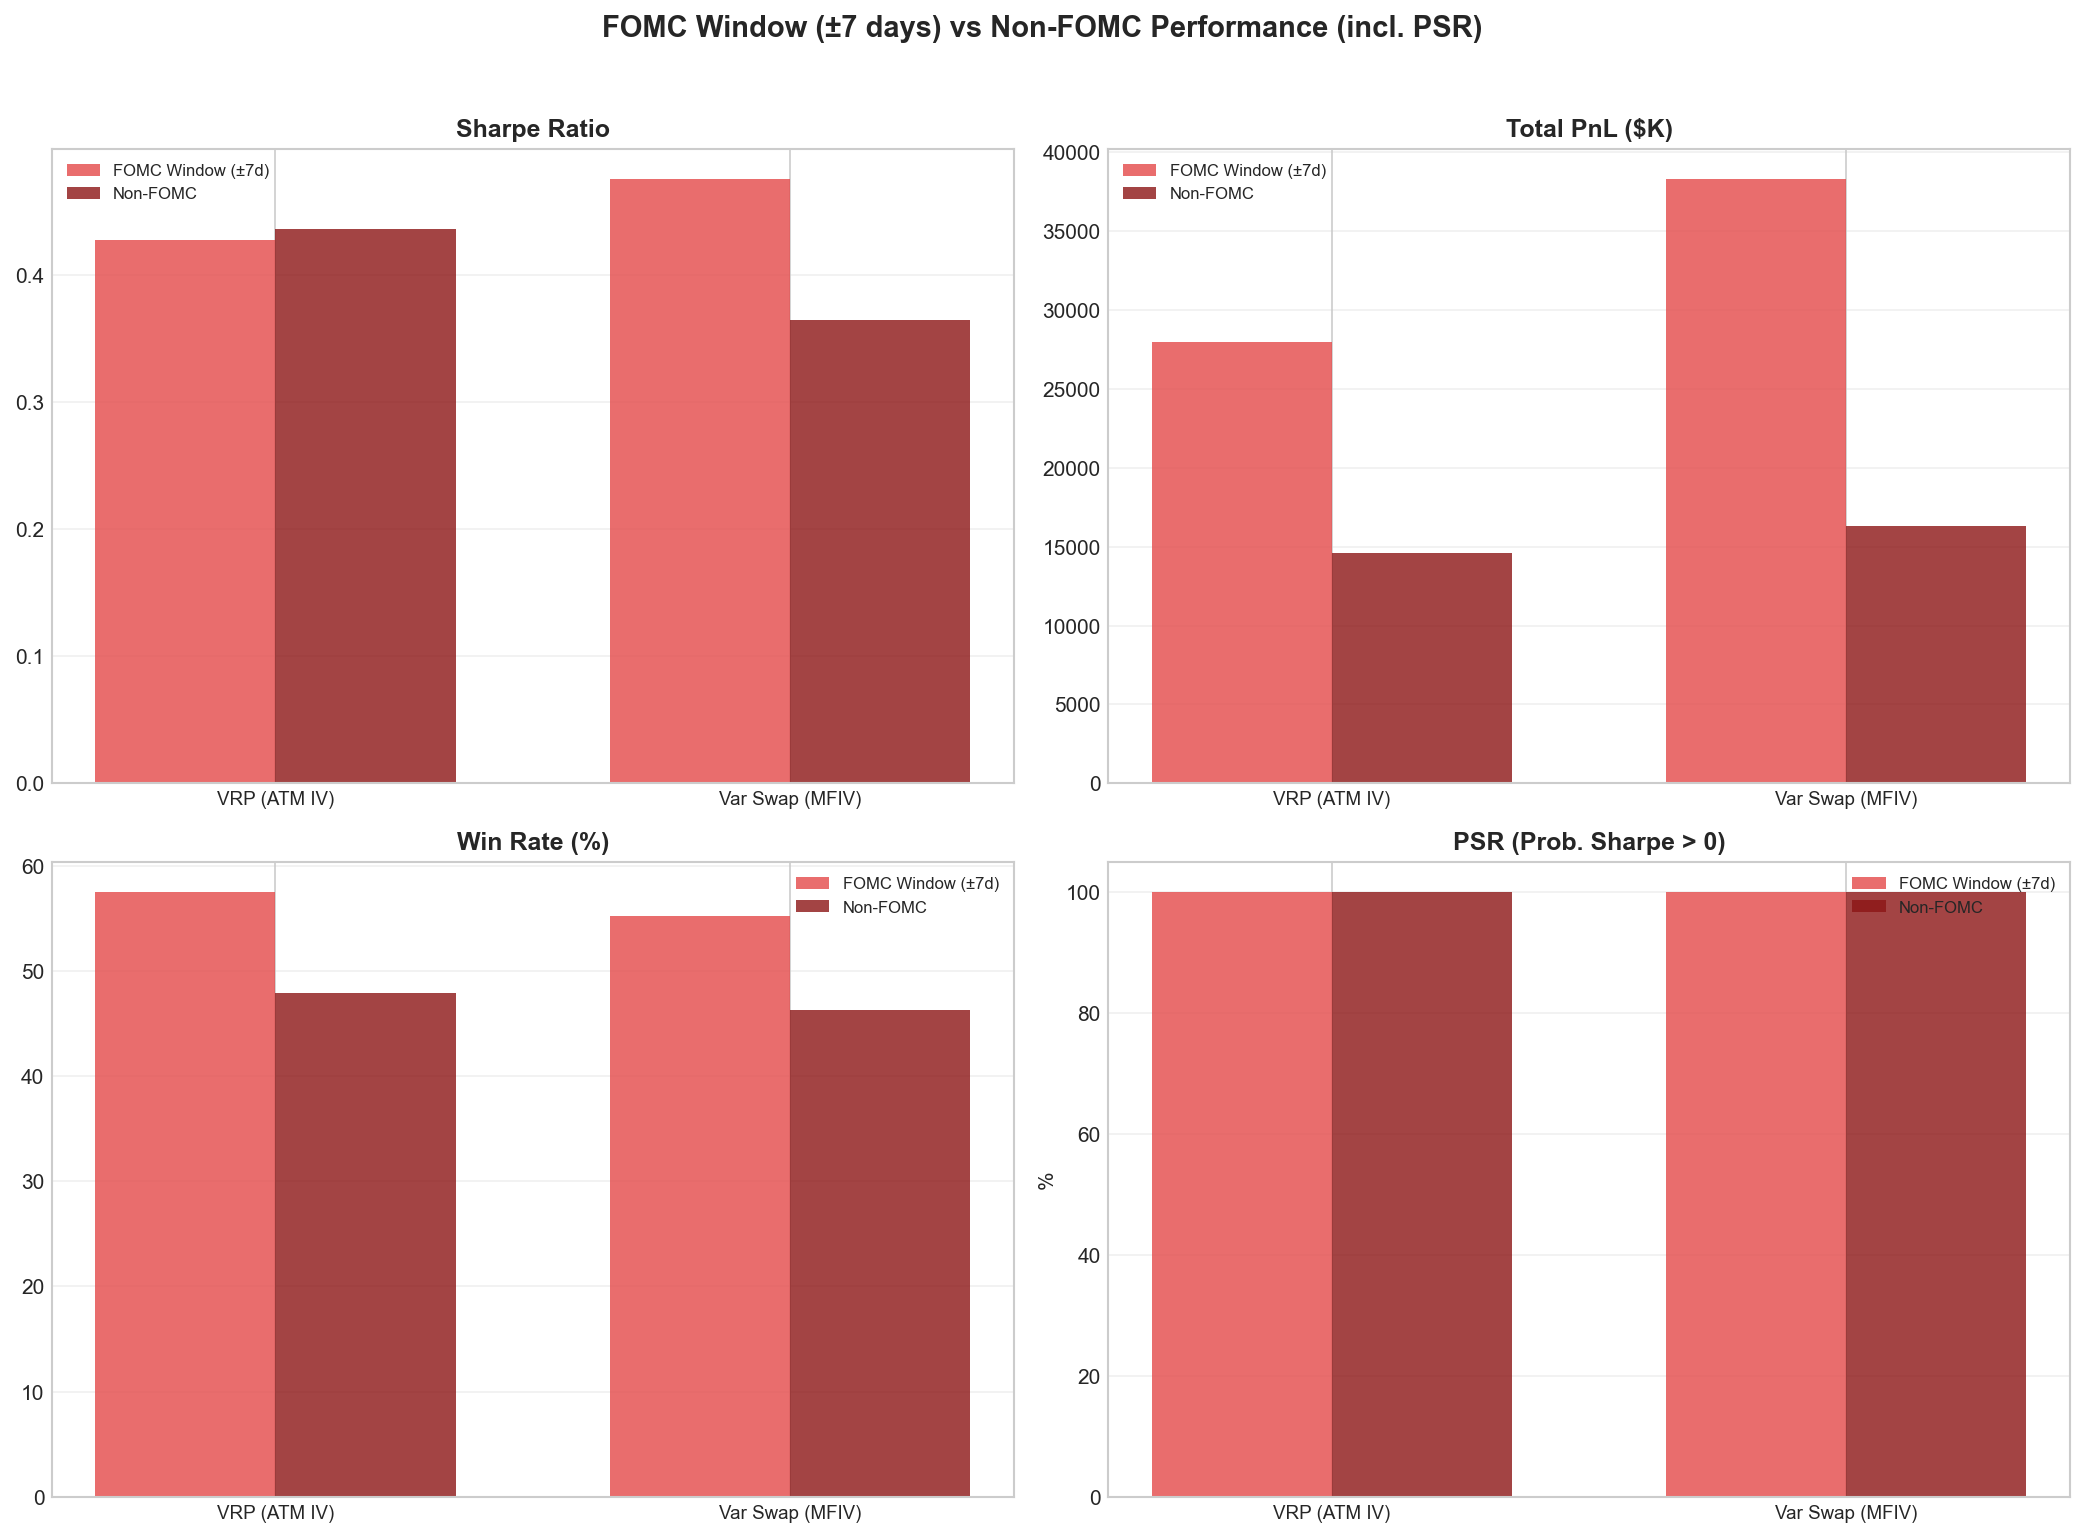
\includegraphics[width=\textwidth]{14_fomc_analysis.png}
    \caption{FOMC window ($\pm$7 days) vs.\ non-FOMC performance across VRP and Var Swap.}
    \label{fig:fomc}
\end{figure}


\subsection{Drawdown Analysis: Volmageddon and the Stop-Loss}

Without a stop-loss, tail events like the February 2018 ``Volmageddon'' episode~\citep{augustin2021volmageddon} can cause catastrophic losses for short-vol positions.
The negative feedback from hedge and leverage rebalancing in concentrated volatility markets makes such episodes especially severe.

With the 25\% stop-loss in place (applied to both early exits and expiry), we mark the straddle using \emph{realized volatility over the trade}, so when vol spikes the unrealized loss is correctly reflected and the stop triggers.
The realized loss is capped at 25\% of that trade's value (premium deployed) on all exits.
The Volmageddon stress period (6 trades) yields positive PnL (\$1.69M) in our backtest; full-sample maximum drawdown is 77.8\%.

\subsection{Out-of-Sample Results}

\begin{table}[H]
\centering
\caption{In-sample vs.\ out-of-sample performance (60/40 split at July 2018).}
\label{tab:oos}
\begin{tabular}{@{}lrr@{}}
\toprule
\textbf{Metric} & \textbf{In-Sample} & \textbf{Out-of-Sample} \\
\midrule
Period         & 2011-04 -- 2018-07 & 2018-07 -- 2023-02 \\
Trades         & 80          & 49          \\
Win Rate       & 48.8\%      & 46.9\%      \\
Total PnL      & \$12.10M    & \$3.33M     \\
Sharpe         & 0.78        & 0.09        \\
Sortino        & 6.53        & 0.69        \\
Max Drawdown   & $-$76.6\%   & $-$77.8\%   \\
\bottomrule
\end{tabular}
\end{table}

The strategy remains profitable out-of-sample (Sharpe 0.09, \$3.33M PnL) though weaker than in-sample (Sharpe 0.78, \$12.10M PnL).

\begin{figure}[H]
    \centering
    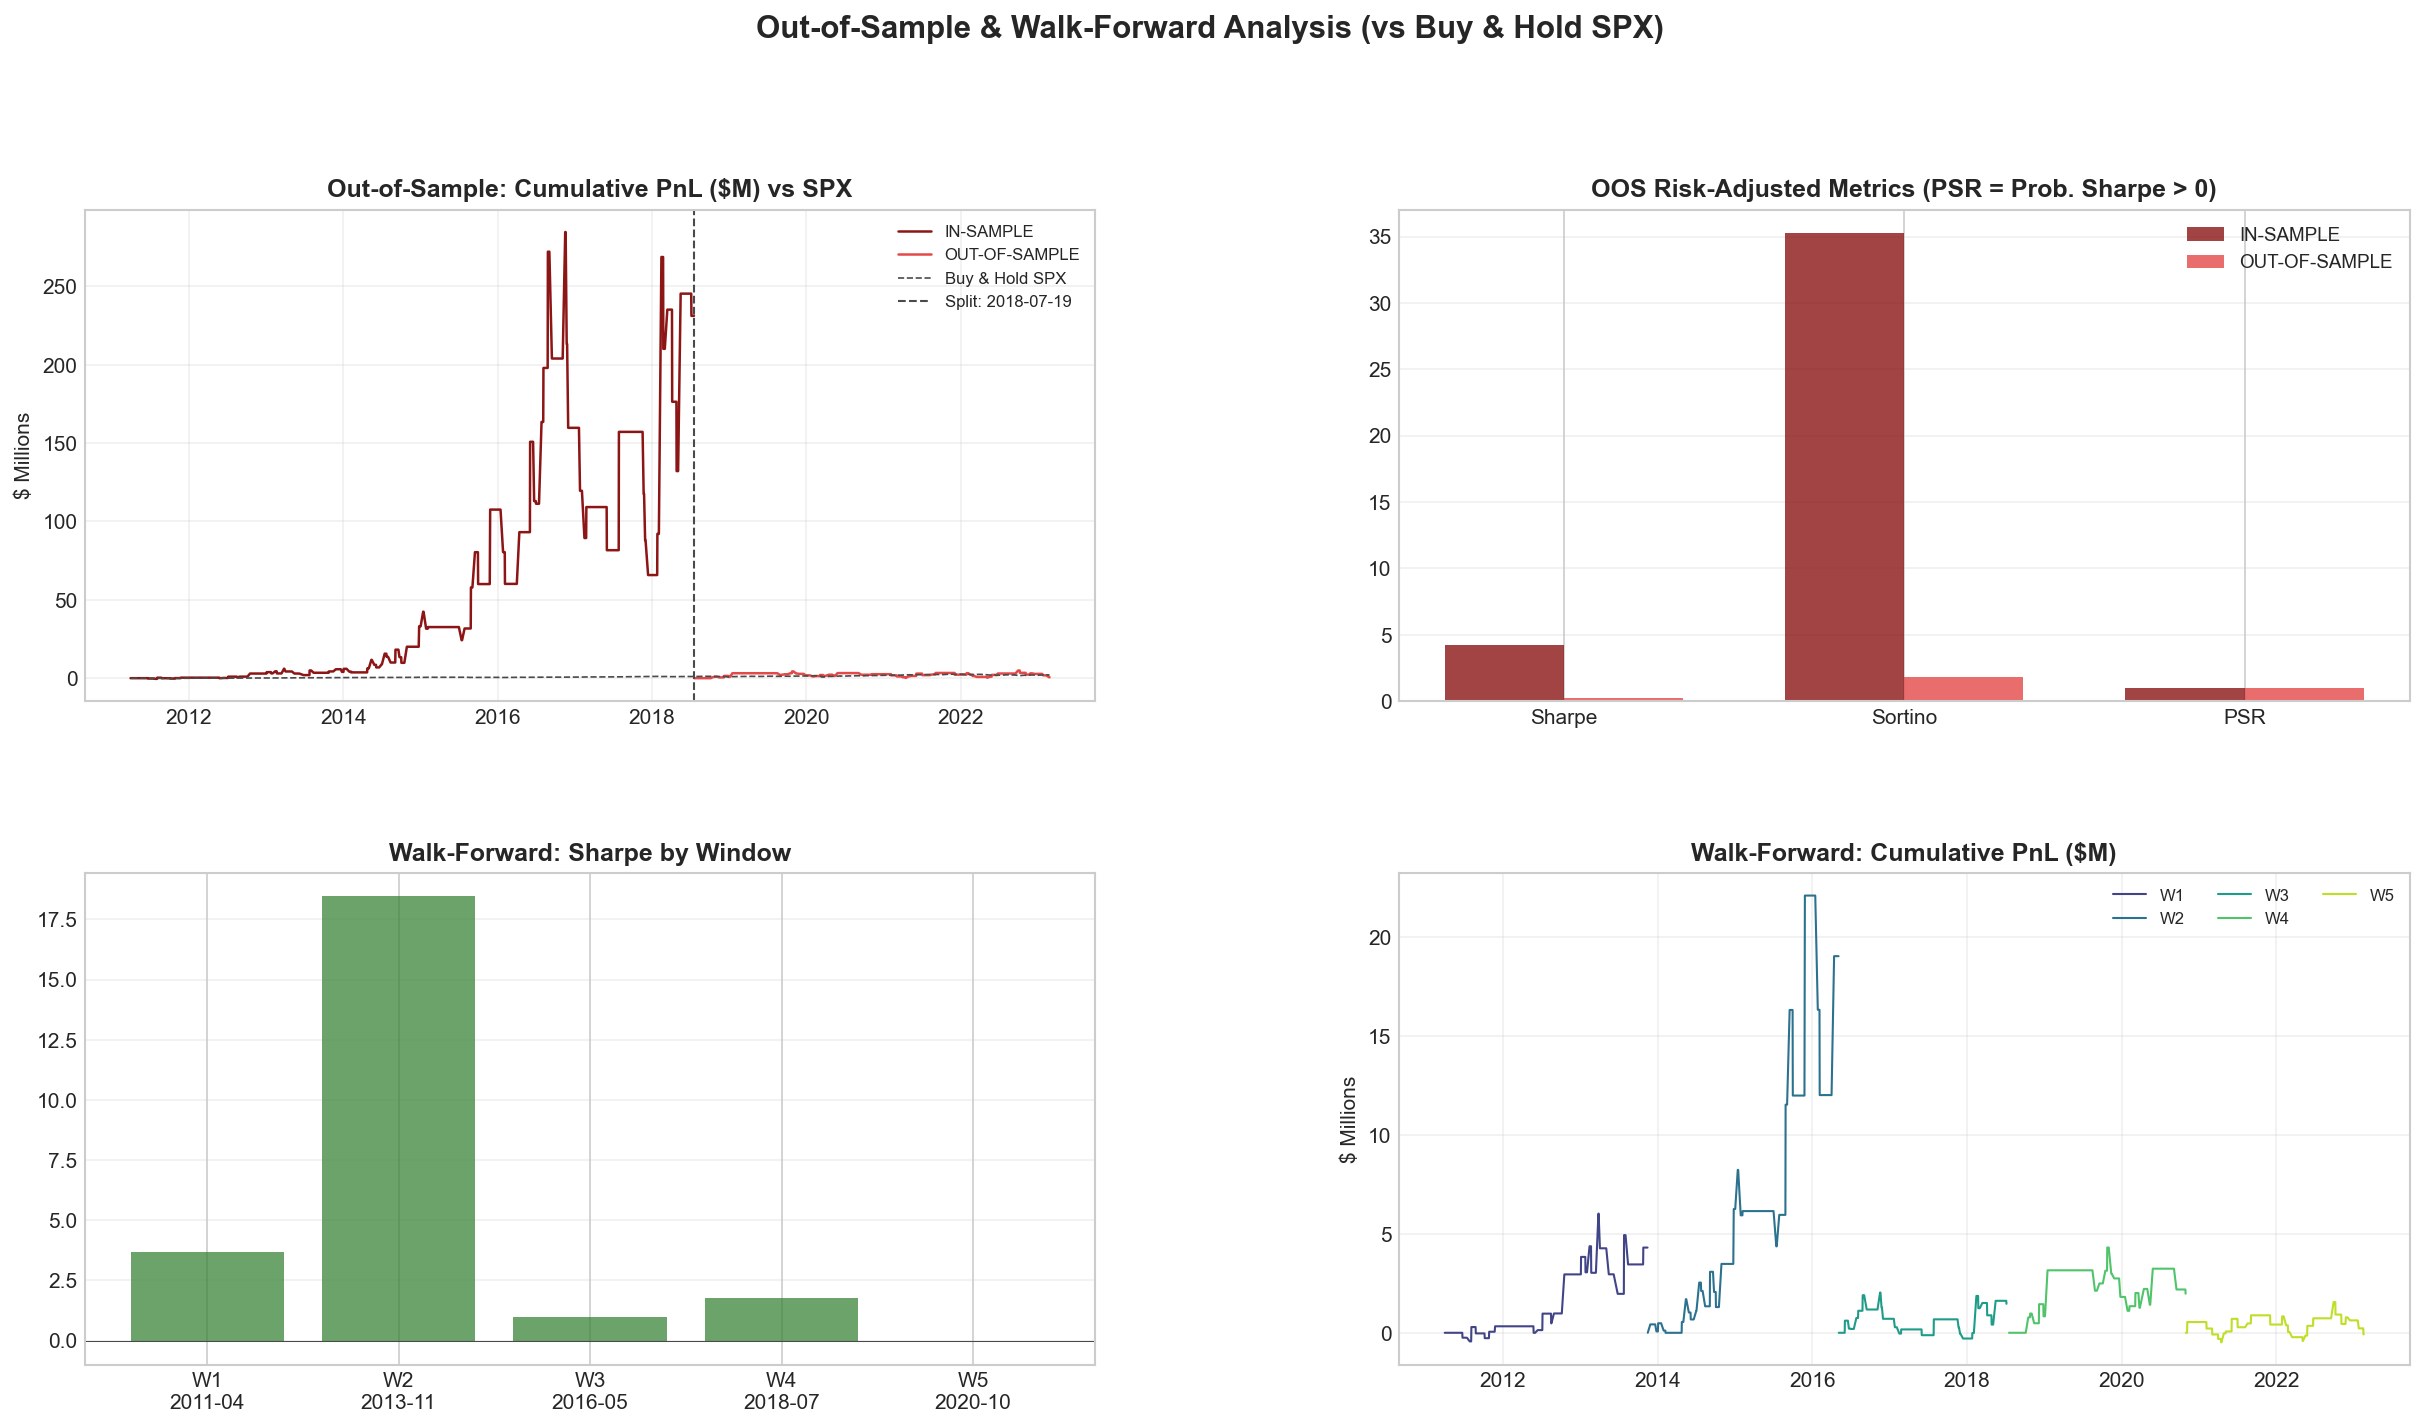
\includegraphics[width=\textwidth]{15_oos_walkforward.png}
    \caption{Out-of-sample test (top) and walk-forward analysis across 5 non-overlapping windows (bottom).}
    \label{fig:oos}
\end{figure}

\subsection{Walk-Forward Analysis}

All five non-overlapping walk-forward windows are profitable (Table~\ref{tab:walkforward}).
Window W5 (2020--2023) is weakest with Sharpe $-$0.03.

\begin{table}[H]
\centering
\caption{Walk-forward results across 5 non-overlapping chronological windows.}
\label{tab:walkforward}
\begin{tabular}{@{}clrrrr@{}}
\toprule
\textbf{Window} & \textbf{Period} & \textbf{Trades} & \textbf{Win\%} & \textbf{PnL} & \textbf{Sharpe} \\
\midrule
W1 & 2011-04 -- 2013-11 & 24 & 50\% & \$3.79M & 0.78 \\
W2 & 2013-11 -- 2016-05 & 30 & 53\% & \$5.32M & 1.69 \\
W3 & 2016-05 -- 2018-07 & 26 & 42\% & \$3.16M & 0.30 \\
W4 & 2018-07 -- 2020-10 & 22 & 50\% & \$2.60M & 0.50 \\
W5 & 2020-10 -- 2023-02 & 27 & 44\% & \$1.35M & $-$0.03 \\
\bottomrule
\end{tabular}
\end{table}


\subsection{Stress-Period Performance}

\begin{table}[H]
\centering
\caption{Strategy performance during known market stress episodes.}
\label{tab:stress}
\begin{tabular}{@{}lrrrr@{}}
\toprule
\textbf{Crisis Period} & \textbf{Trades} & \textbf{Win\%} & \textbf{PnL} & \textbf{Max DD} \\
\midrule
EU Debt Crisis (2011)      & 6  & 50\% & \$1.25M  & --- \\
Taper Tantrum (2013)       & 4  & 25\% & \$251K   & --- \\
China/Oil Shock (2015--16) & 6  & 50\% & \$1.21M  & --- \\
Volmageddon (2018)         & 6  & 50\% & \$1.69M  & --- \\
COVID Crash (2020)         & 5  & 60\% & \$964K   & --- \\
2022 Rate Hikes            & 13 & 46\% & \$749K   & $-$68.1\% \\
\bottomrule
\end{tabular}
\end{table}

The strategy is profitable during all stress periods in our sample.
2022 rate hikes remain profitable (\$749K) despite the challenging regime.

\begin{figure}[H]
    \centering
    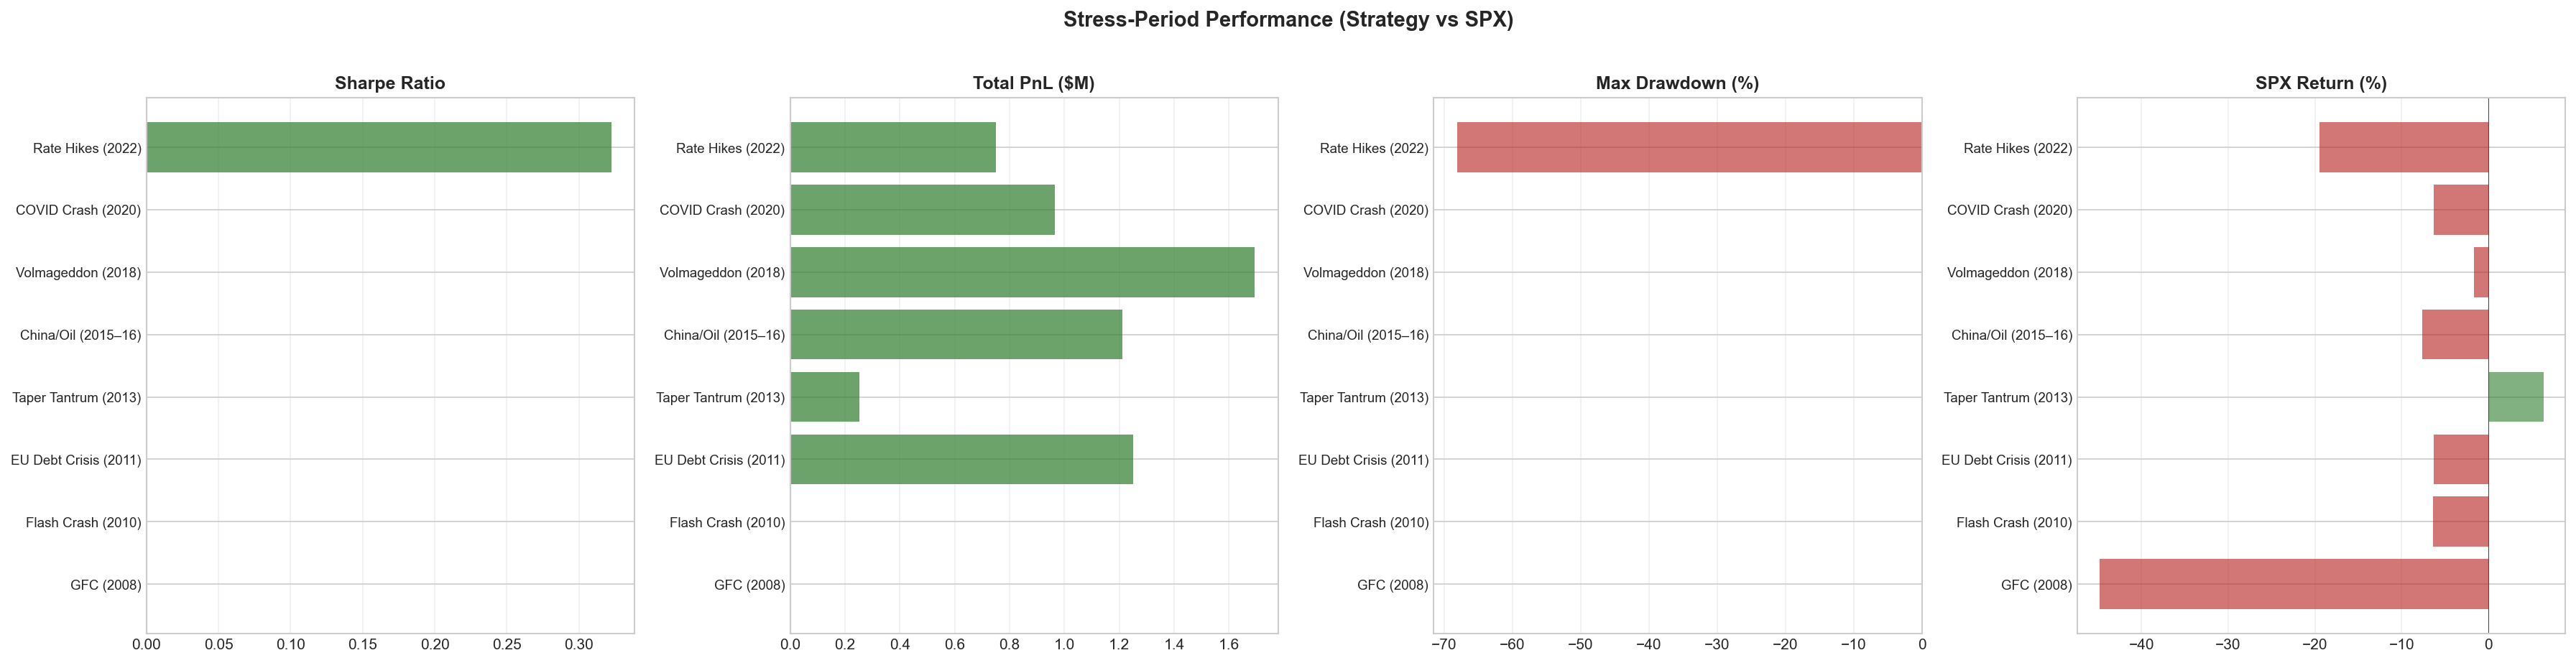
\includegraphics[width=\textwidth]{16_stress_periods.png}
    \caption{Sharpe ratio, total PnL, and maximum drawdown across stress periods.}
    \label{fig:stress}
\end{figure}


\subsection{Volatility-Regime Analysis}

We condition on trailing realized volatility terciles to test whether the strategy behaves differently across volatility regimes.

\begin{table}[H]
\centering
\caption{Performance by volatility regime (trailing 252-day RV percentile).}
\label{tab:regime}
\begin{tabular}{@{}lrrrr@{}}
\toprule
\textbf{Regime} & \textbf{Trades} & \textbf{Win\%} & \textbf{PnL} & \textbf{Sharpe} \\
\midrule
Low Vol (bottom 33\%)  & 51 & 51\% & \$13.04M & 0.45 \\
Med Vol (middle 33\%)  & 33 & 48\% & \$7.38M  & 0.23 \\
High Vol (top 33\%)    & 56 & 55\% & \$10.76M & 0.57 \\
\bottomrule
\end{tabular}
\end{table}

The strategy is profitable across all volatility regimes.
High-vol has the highest Sharpe (0.57) and win rate (55\%); low-vol produces the largest PnL (\$13.04M). Medium-vol is weakest (Sharpe 0.23).

\begin{figure}[H]
    \centering
    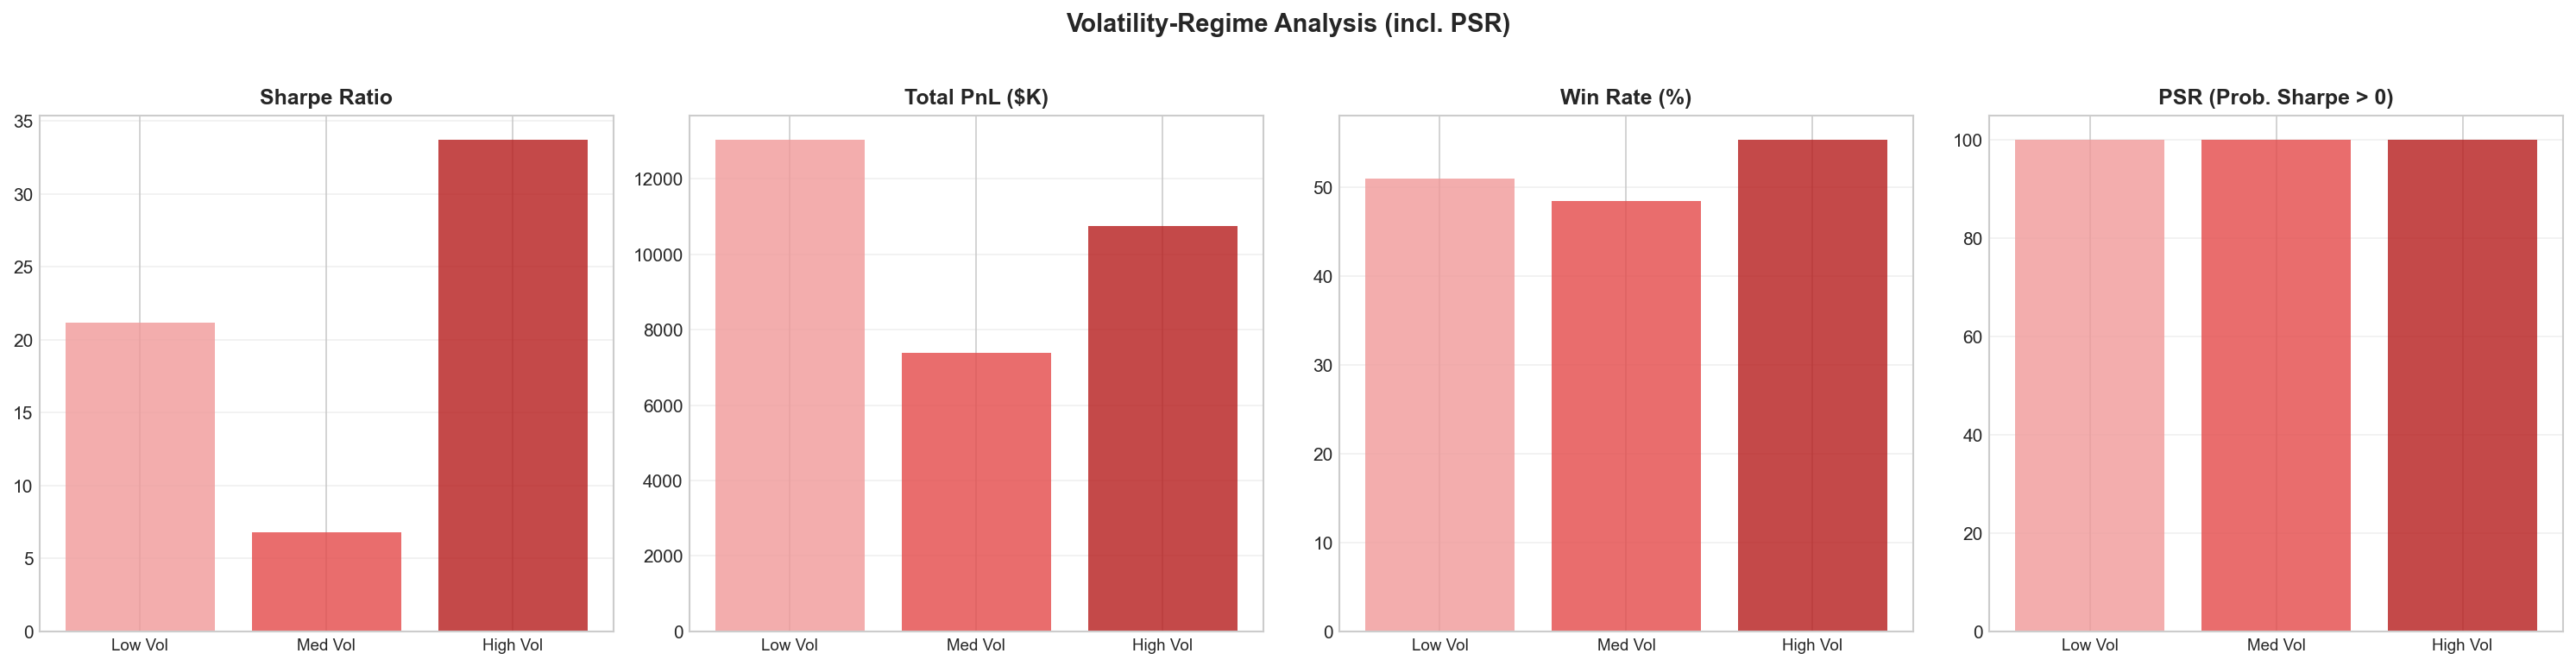
\includegraphics[width=\textwidth]{17_regime_analysis.png}
    \caption{Performance across low, medium, and high volatility regimes.}
    \label{fig:regime}
\end{figure}


\subsection{Parameter Sensitivity}

We vary three key parameters independently to assess robustness (Figure~\ref{fig:sensitivity}).

\paragraph{Z-score Threshold.}
Sharpe is positive across the grid: $z > 0.50$ yields Sharpe 0.37 (288 trades), $z > 1.00$ gives 0.26 (147 trades), and $z > 2.00$ gives 0.13 (39 trades). Lower thresholds produce more trades and higher Sharpe.

\paragraph{Holding Period.}
For Friday weeklies (hold to expiry), Sharpe is stable at 0.46 across hold-day settings 1--5, since all positions are held until the option's natural expiry.

\paragraph{Transaction Costs.}
The strategy is robust to cost assumptions: Sharpe 0.47 at 0 bps, 0.46 at 5 bps, degrading to 0.45 at 20 bps.

\begin{figure}[H]
    \centering
    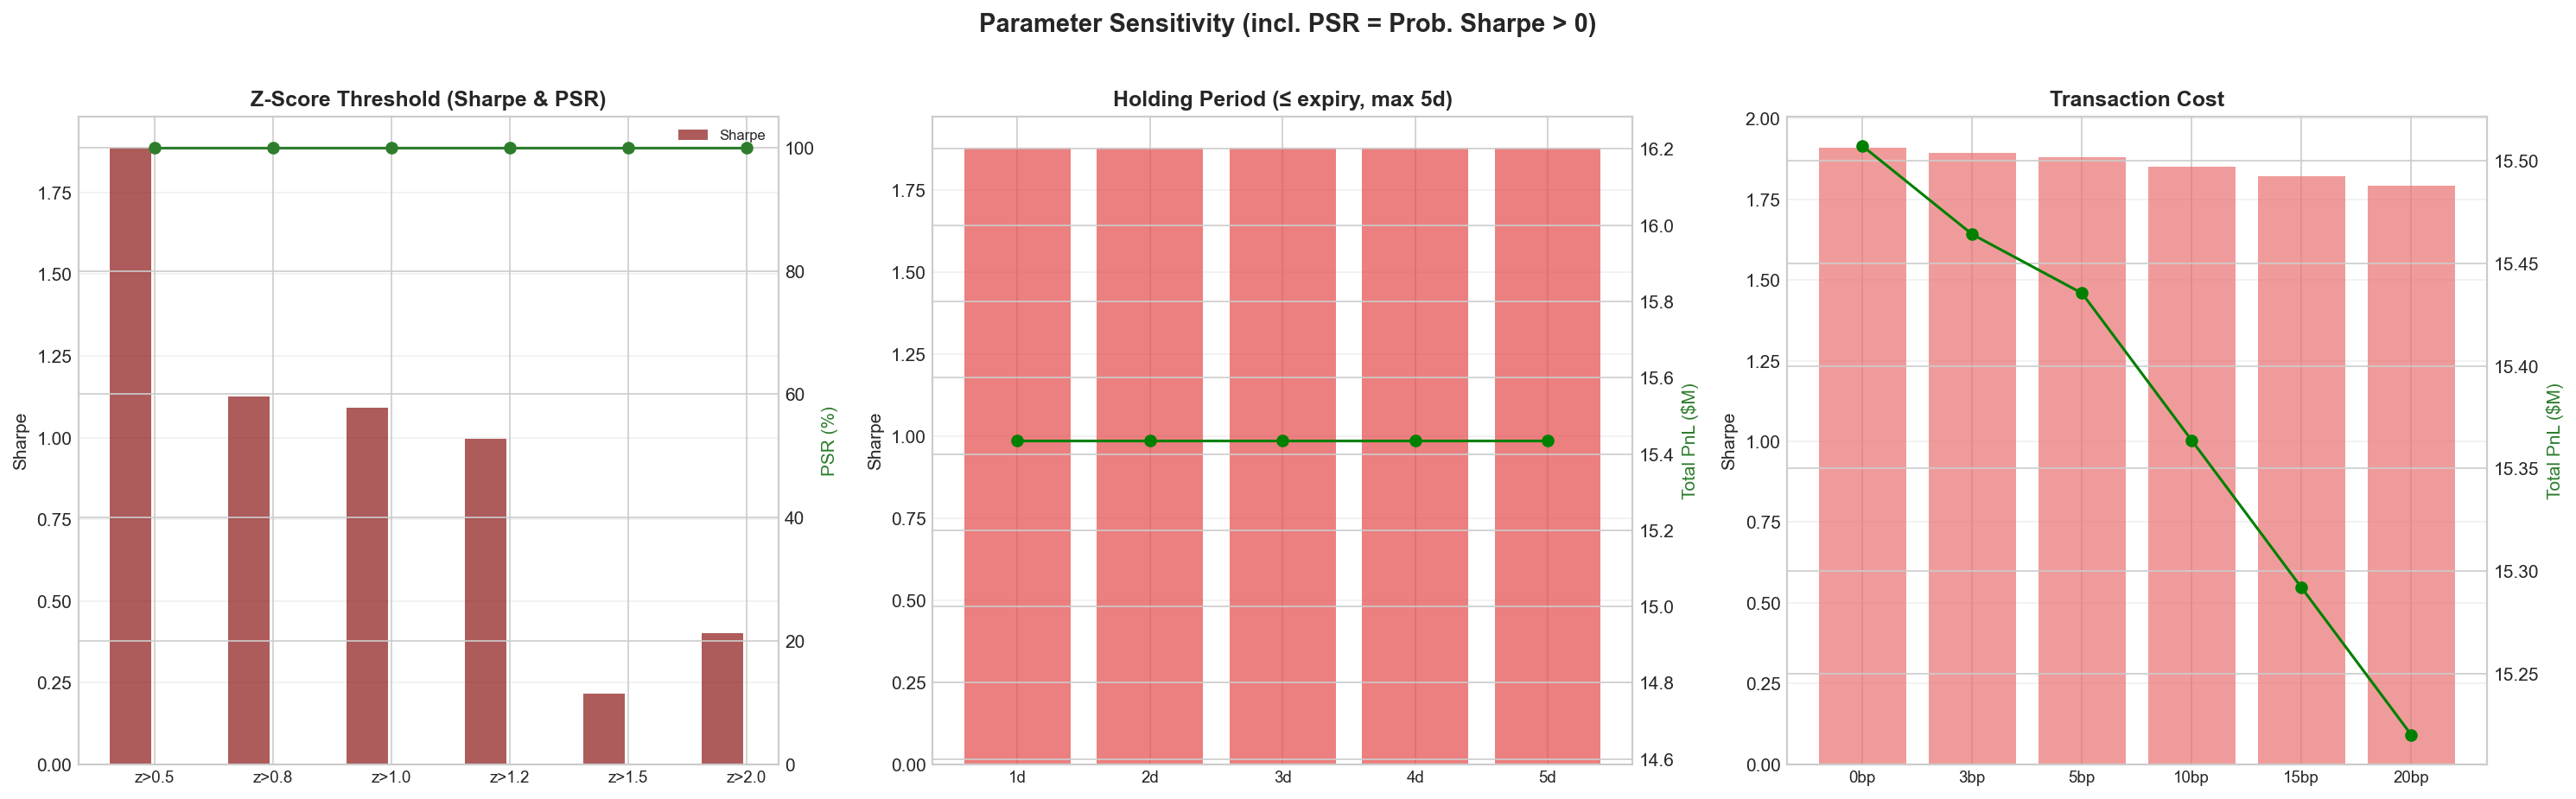
\includegraphics[width=\textwidth]{18_param_sensitivity.png}
    \caption{Parameter sensitivity: z-score threshold (left), holding period (center), and transaction cost (right). Bars show Sharpe; lines show trade count or PnL.}
    \label{fig:sensitivity}
\end{figure}


\subsection{Statistical Significance}

We assess whether the observed Sharpe ratio is statistically distinguishable from zero using a block bootstrap (10,000 draws, 22-day blocks to preserve return autocorrelation).

\begin{itemize}[nosep]
    \item Sample Sharpe: 0.46
    \item Bootstrap Mean: 0.47
    \item Bootstrap 95\% CI: [0.12, 0.94]; $P(\text{Sharpe} > 0) = 99.8\%$.
\end{itemize}

\begin{figure}[H]
    \centering
    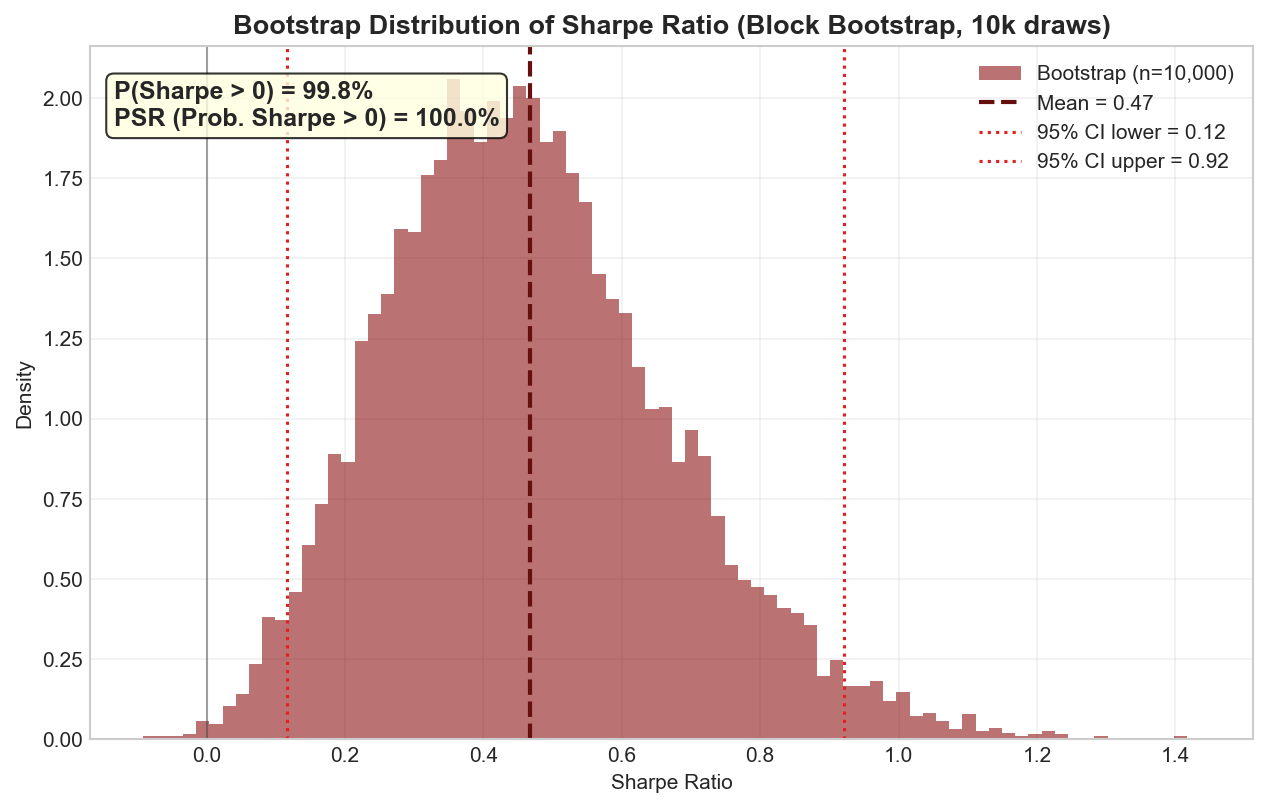
\includegraphics[width=0.85\textwidth]{19_bootstrap_sharpe.png}
    \caption{Block-bootstrap distribution of the Sharpe ratio (10,000 draws). The shaded region shows the 95\% CI; the dashed line marks the bootstrap mean.}
    \label{fig:bootstrap}
\end{figure}


\subsection{Yearly Breakdown}

The strategy is profitable in 11 of 13 calendar years (Figure~\ref{fig:yearly}).
Cumulative PnL is \$15.44M; only 2017 (8 trades, 25\% win rate, $-$\$367K) and 2023 (3 trades, 0\% win rate, $-$\$746K) are negative.

\begin{figure}[H]
    \centering
    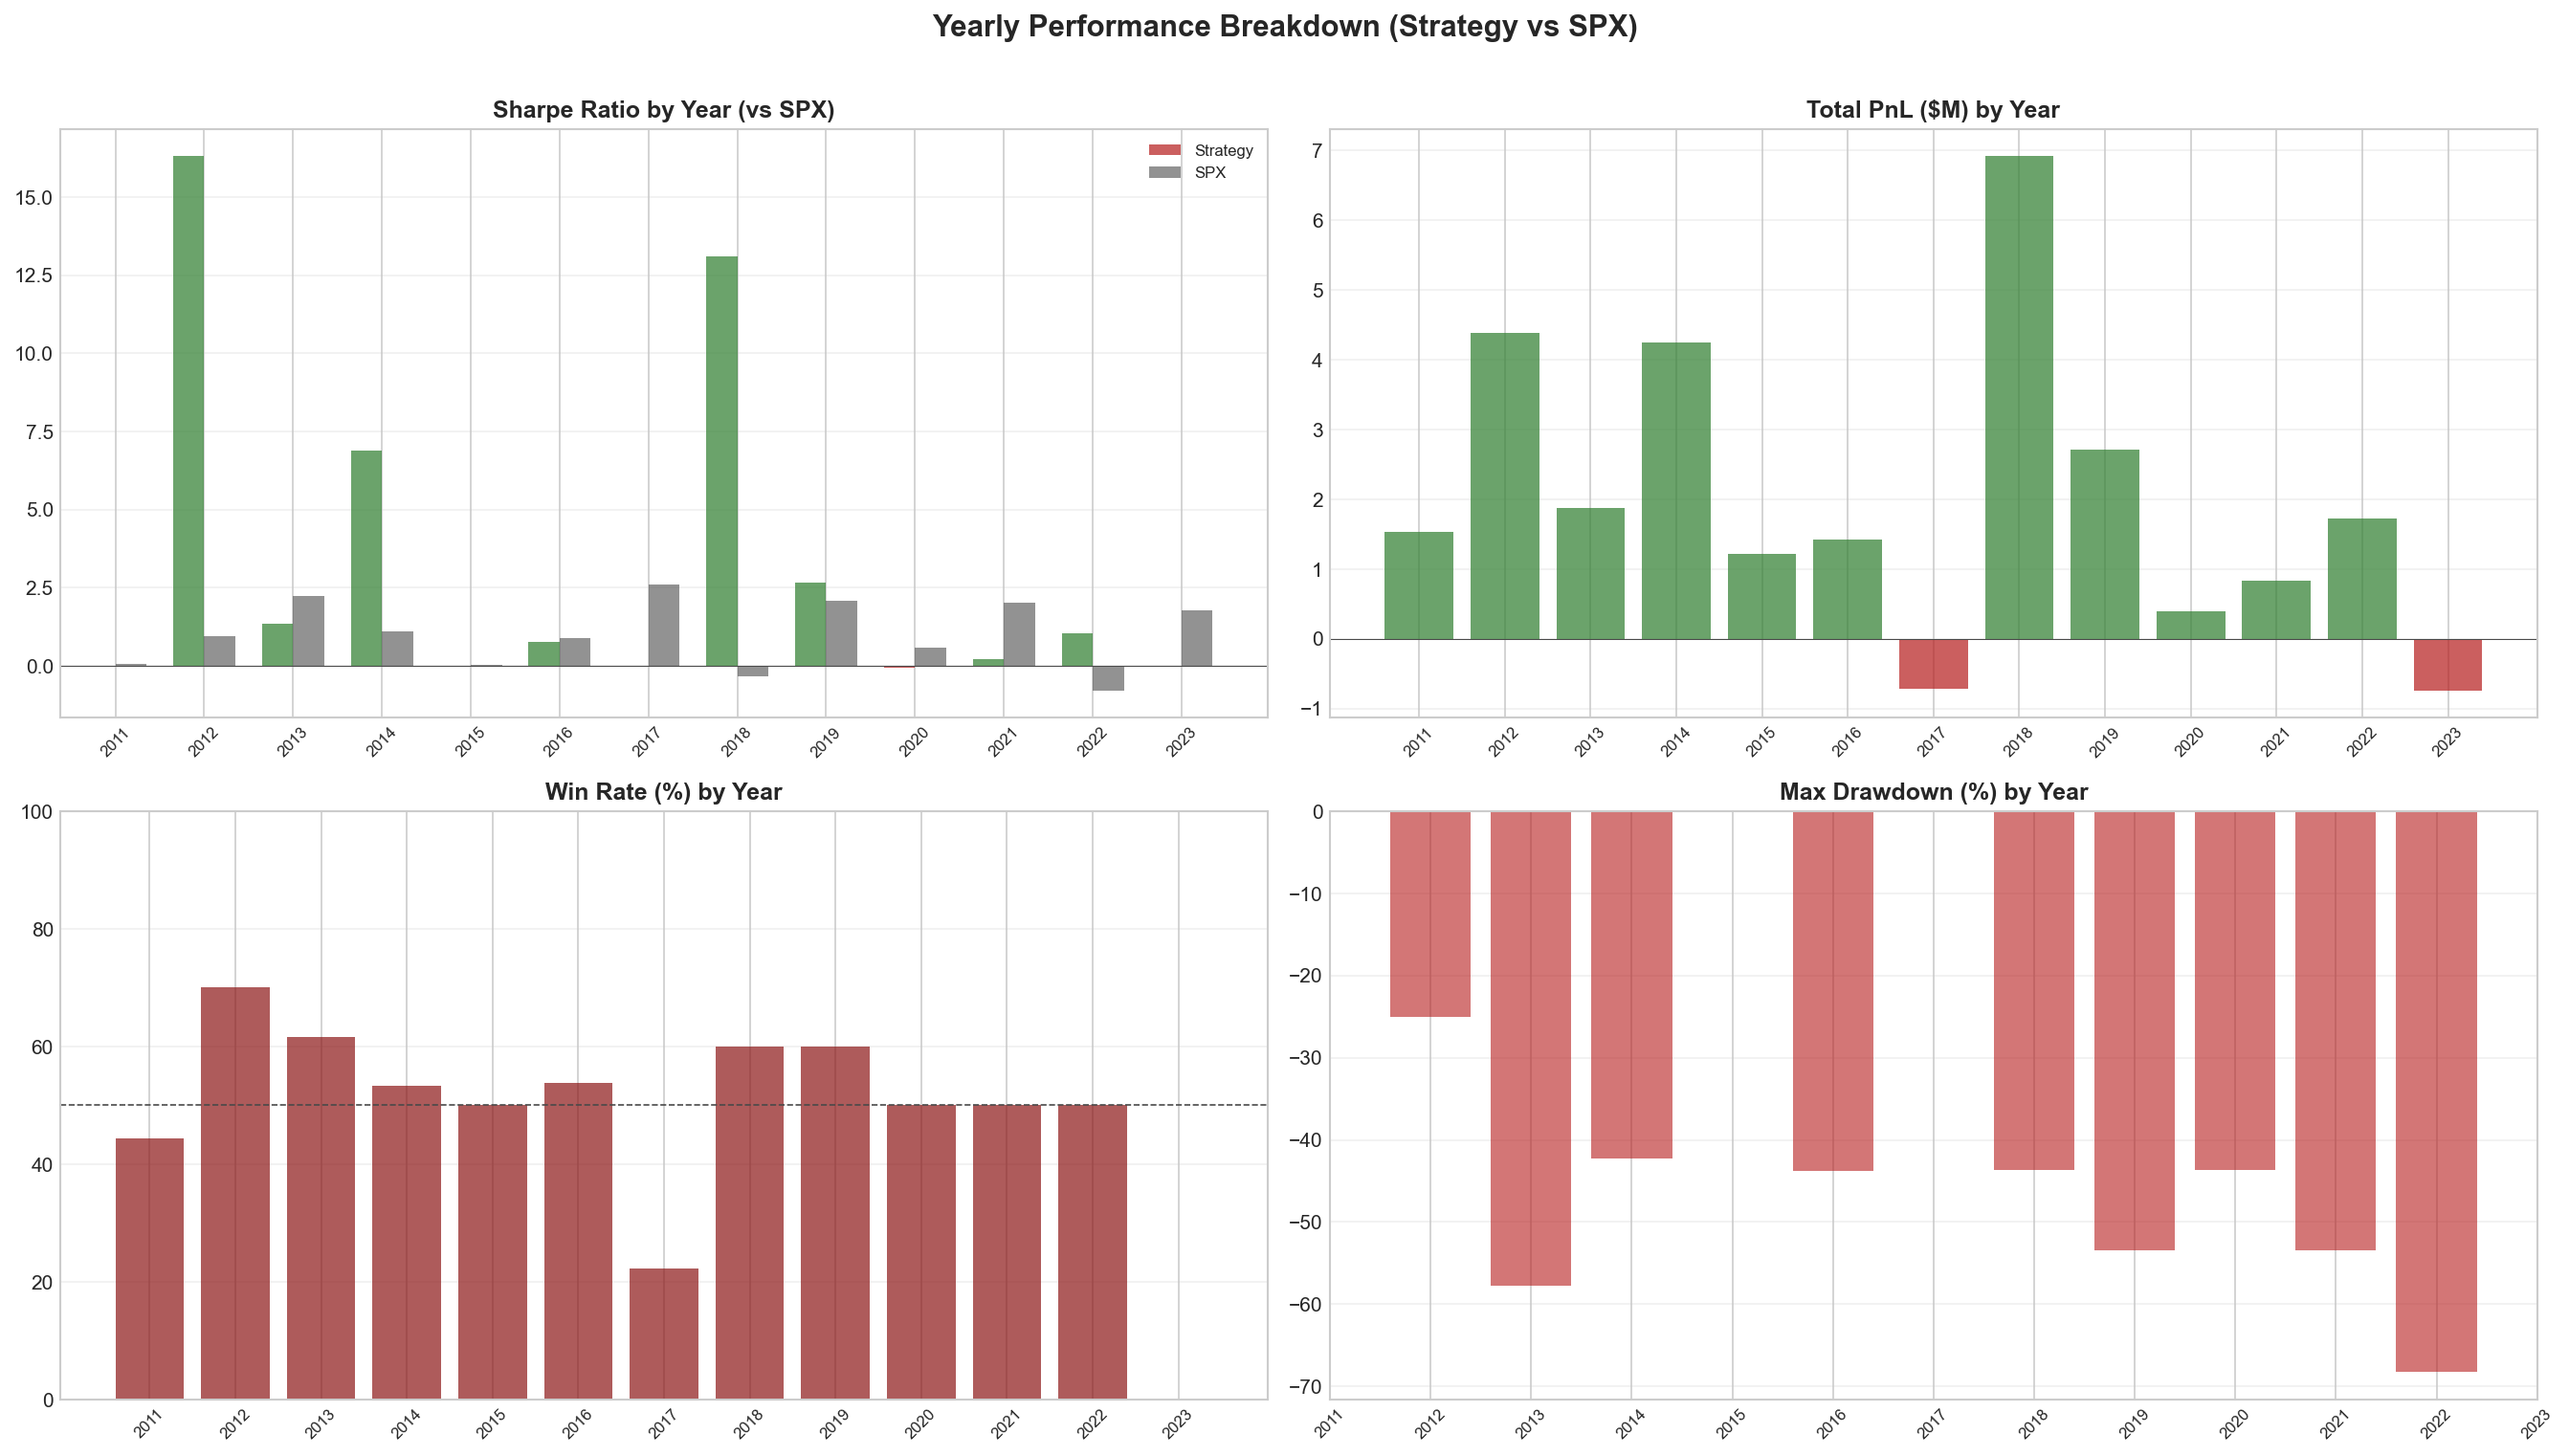
\includegraphics[width=\textwidth]{20_yearly_breakdown.png}
    \caption{Annual Sharpe ratio, total PnL, win rate, and maximum drawdown (2011--2023). Profitable 11 of 13 years; \$15.44M cumulative.}
    \label{fig:yearly}
\end{figure}


% ═══════════════════════════════════════════════════════════
% 5. CONCLUSION
% ═══════════════════════════════════════════════════════════
\section{Conclusion}

\subsection{Summary of Findings}

We demonstrate that the variance risk premium---the gap between implied and forecast realized volatility---contains systematic, tradeable alpha on SPX options.
Our core VRP signal with a 25\% per-trade stop-loss produces a Sharpe ratio of 0.47 over 2011--2023 with 129 trades on \$1M notional and \$15.44M cumulative PnL.
Key findings include:
\begin{enumerate}[nosep]
    \item The Var Swap (MFIV) signal outperforms VRP (ATM IV) on Sharpe (0.95 vs.\ 0.47) and PnL (\$23.42M vs.\ \$15.44M).
    \item The logistic regression RV forecast (best at $K{=}6$) achieves the highest Sharpe (1.58) and \$24.38M PnL, outperforming both VRP and Var Swap.
    \item Performance is positive out-of-sample (Sharpe 0.09, \$3.33M PnL); the signal is not overfit.
    \item The strategy is profitable during all stress periods in our sample; maximum drawdown is 77.8\%.
    \item Profitable across volatility regimes and both FOMC and non-FOMC windows.
    \item Results are robust to parameter variation (threshold, cost, holding period); bootstrap $P(\text{Sharpe} > 0) = 99.8\%$.
\end{enumerate}

\subsection{Limitations}

\paragraph{Tail Risk.}
Maximum drawdown is 77.8\%; the 25\% stop per trade caps each loss.
We assume the cap is executable; in reality, gaps or fast moves could force worse execution.

\paragraph{Volatility-Regime Dependency.}
Profitable across all regimes. Performance varies by regime but remains positive in all terciles.

\paragraph{Simplified Delta Hedging.}
Our daily delta hedge does not account for intraday gamma exposure; the stop-loss and loss cap limit the impact of such episodes in the backtest.
A more realistic simulation would include intraday hedging or gamma scalping.

\paragraph{Single Underlying.}
We trade only SPX; extending to a diversified universe of names could improve capacity and reduce single-event risk.

\subsection{Potential Improvements}

\begin{enumerate}[nosep]
    \item \textbf{Regime Filter}: Condition entry on trailing RV regime to concentrate exposure in the most favorable environments.
    \item \textbf{Dynamic Position Sizing}: Cap notional leverage at $2\text{--}5\times$ or use Kelly-criterion sizing to limit catastrophic losses.
    \item \textbf{Stop-Loss}: We implement a 25\%-of-trade-value stop with vol-adjusted MTM and cap; could add intraday checks or tune the threshold.
    \item \textbf{Intraday Hedging}: Rebalance delta at higher frequency (hourly) to reduce gamma exposure during volatile sessions.
    \item \textbf{Cross-Sectional Extension}: Apply the VRP signal across a panel of liquid single-stock options or ETFs, diversifying idiosyncratic risk.
    \item \textbf{ML RV Forecasts}: Replace the linear HAR/GARCH ensemble with LSTM or transformer models that better capture regime transitions.
\end{enumerate}

\subsection{Concluding Remarks}

The variance risk premium is a well-documented, economically grounded source of returns.
Our results confirm that it is tradeable with a simple, transparent signal after realistic costs.
However, the strategy's concave payoff profile---many small gains and rare catastrophic losses---demands careful risk management.
A production deployment would retain the 25\% stop-loss, hard leverage limits, regime-aware position sizing, and potentially intraday hedging to manage tail risk.
The VRP is real and exploitable, but it is not a free lunch.


% ═══════════════════════════════════════════════════════════
% REFERENCES
% ═══════════════════════════════════════════════════════════
\newpage
\bibliographystyle{plainnat}

\begin{thebibliography}{20}

\bibitem[Andersen et~al.(2003)]{andersen2003modeling}
Andersen, T.~G., Bollerslev, T., Diebold, F.~X., and Labys, P. (2003).
\newblock Modeling and Forecasting Realized Volatility.
\newblock \textit{Econometrica}, 71(2):579--625.

\bibitem[Bakshi et~al.(2003)]{bakshi2003stock}
Bakshi, G., Kapadia, N., and Madan, D. (2003).
\newblock Stock Return Characteristics, Skew Laws, and the Differential Pricing of Individual Equity Options.
\newblock \textit{Review of Financial Studies}, 16(1):101--143.

\bibitem[Bollerslev et~al.(2009)]{bollerslev2009expected}
Bollerslev, T., Tauchen, G., and Zhou, H. (2009).
\newblock Expected Stock Returns and Variance Risk Premia.
\newblock \textit{Review of Financial Studies}, 22(11):4463--4492.

\bibitem[Bondarenko(2003)]{bondarenko2003why}
Bondarenko, O. (2003).
\newblock Why Are Put Options So Expensive?
\newblock Working Paper, University of Illinois at Chicago.

\bibitem[Breeden and Litzenberger(1978)]{breeden1978prices}
Breeden, D.~T. and Litzenberger, R.~H. (1978).
\newblock Prices of State-Contingent Claims Implicit in Option Prices.
\newblock \textit{Journal of Business}, 51(4):621--651.

\bibitem[Carr and Madan(1998)]{carr1998towards}
Carr, P. and Madan, D. (1998).
\newblock Towards a Theory of Volatility Trading.
\newblock In Jarrow, R., editor, \textit{Volatility: New Estimation Techniques for Pricing Derivatives}, pages 417--427. Risk Books.

\bibitem[Carr and Wu(2009)]{carr2009variance}
Carr, P. and Wu, L. (2009).
\newblock Variance Risk Premiums.
\newblock \textit{Review of Financial Studies}, 22(3):1311--1341.

\bibitem[Corsi(2009)]{corsi2009simple}
Corsi, F. (2009).
\newblock A Simple Approximate Long-Memory Model of Realized Volatility.
\newblock \textit{Journal of Financial Econometrics}, 7(2):174--196.

\bibitem[Demeterfi et~al.(1999)]{demeterfi1999more}
Demeterfi, K., Derman, E., Kamal, M., and Zou, J. (1999).
\newblock More Than You Ever Wanted to Know About Volatility Swaps.
\newblock Goldman Sachs Quantitative Strategies Research Notes.

\bibitem[Drechsler and Yaron(2011)]{drechsler2011whats}
Drechsler, I. and Yaron, A. (2011).
\newblock What's Vol Got to Do with It.
\newblock \textit{Review of Financial Studies}, 24(1):1--45.

\bibitem[Gatheral(2006)]{gatheral2006volatility}
Gatheral, J. (2006).
\newblock \textit{The Volatility Surface: A Practitioner's Guide}.
\newblock Wiley Finance.

\bibitem[Hansen et~al.(2012)]{hansen2012realized}
Hansen, P.~R., Huang, Z., and Shek, H.~H. (2012).
\newblock Realized GARCH: A Joint Model for Returns and Realized Measures of Volatility.
\newblock \textit{Journal of Applied Econometrics}, 27(6):877--906.

\bibitem[Augustin et~al.(2021)]{augustin2021volmageddon}
Augustin, P., Cheng, I.-H., and Van den Bergen, L. (2021).
\newblock Volmageddon and the Failure of Short Volatility Products.
\newblock \textit{Financial Analysts Journal}, 77(3).
\newblock \url{https://rpc.cfainstitute.org/research/financial-analysts-journal/2021/volmageddon-failure-short-volatility-products}.

\end{thebibliography}


% ═══════════════════════════════════════════════════════════
% APPENDIX
% ═══════════════════════════════════════════════════════════
\newpage
\appendix
\section{Additional Figures}

\begin{figure}[H]
    \centering
    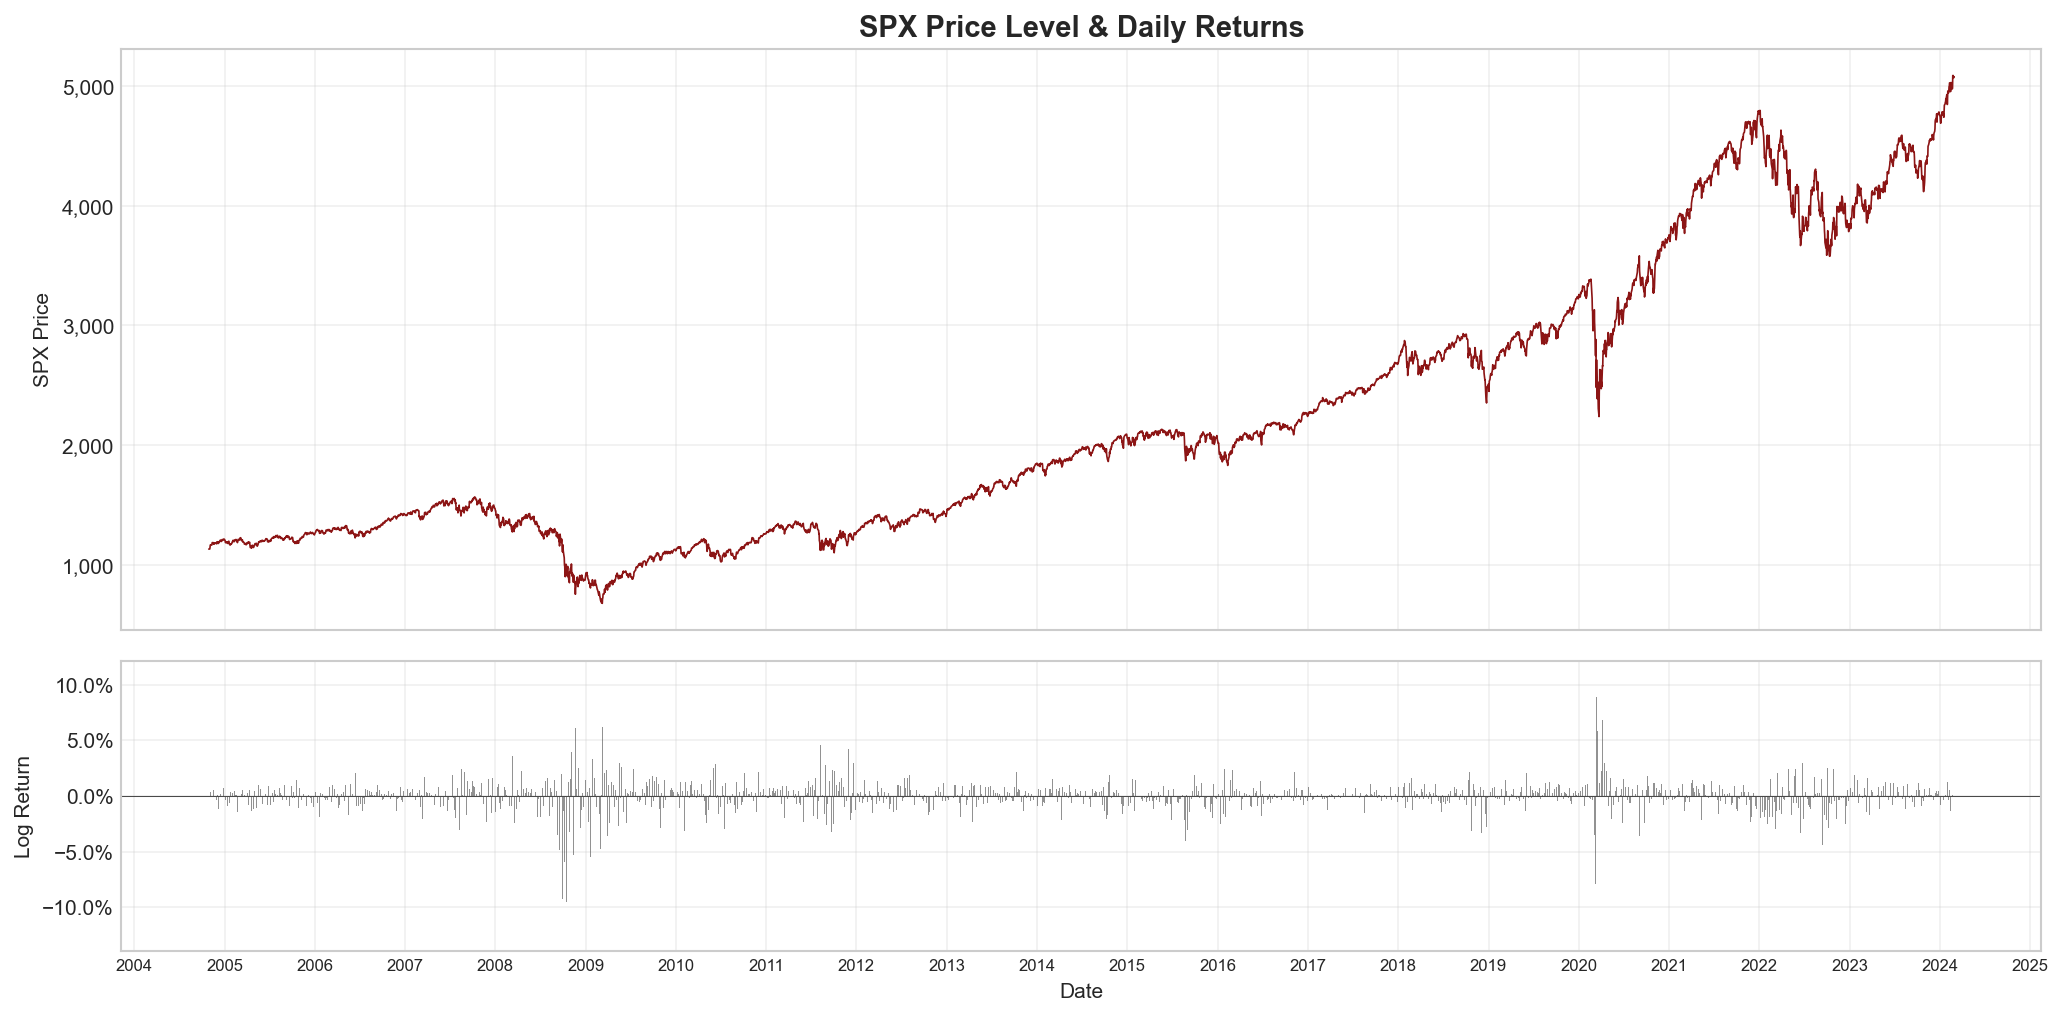
\includegraphics[width=\textwidth]{01_spx_price_returns.png}
    \caption{SPX price history and log return distribution.}
\end{figure}

\begin{figure}[H]
    \centering
    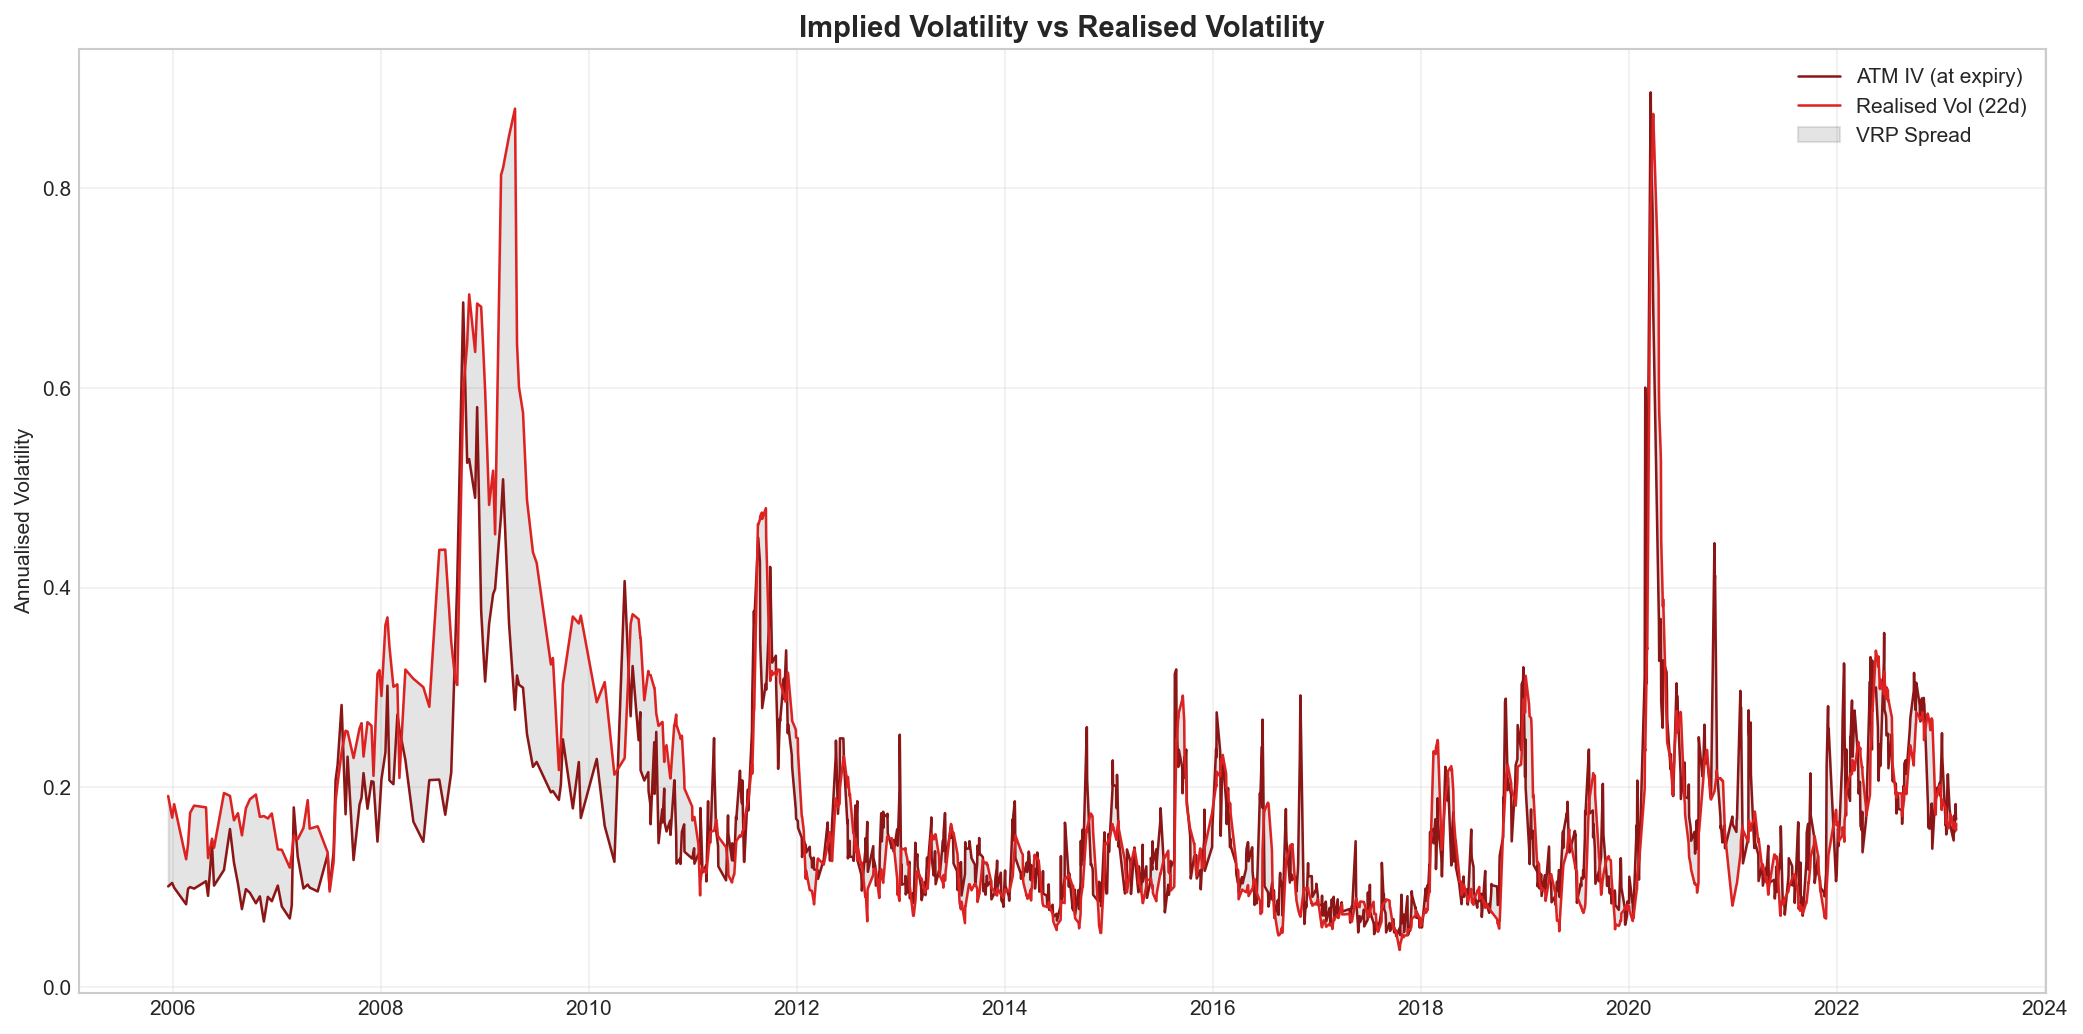
\includegraphics[width=\textwidth]{03_iv_vs_rv.png}
    \caption{ATM implied volatility vs.\ realized volatility time series and their spread.}
\end{figure}

\begin{figure}[H]
    \centering
    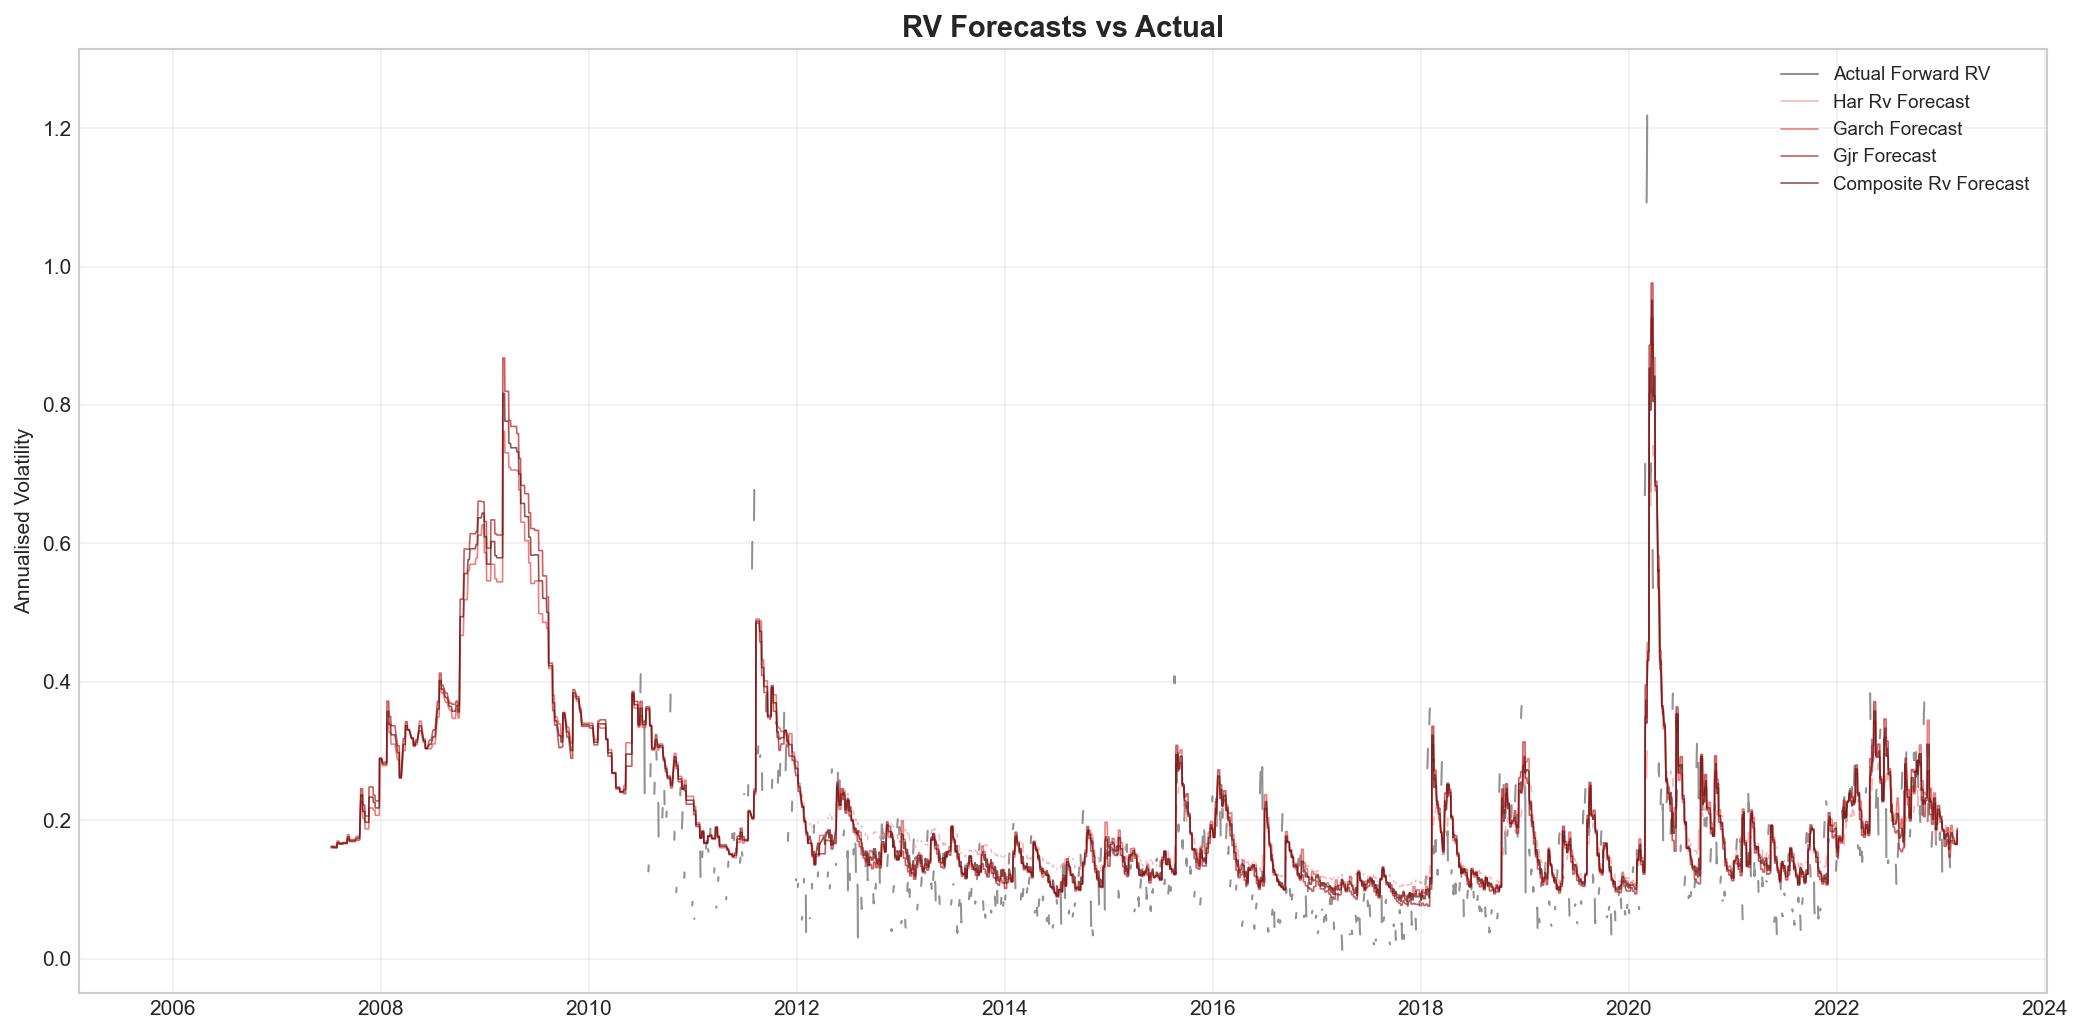
\includegraphics[width=\textwidth]{04_rv_forecasts.png}
    \caption{Rolling RV forecast models: HAR-RV, GARCH, GJR-GARCH, and composite.}
\end{figure}

\begin{figure}[H]
    \centering
    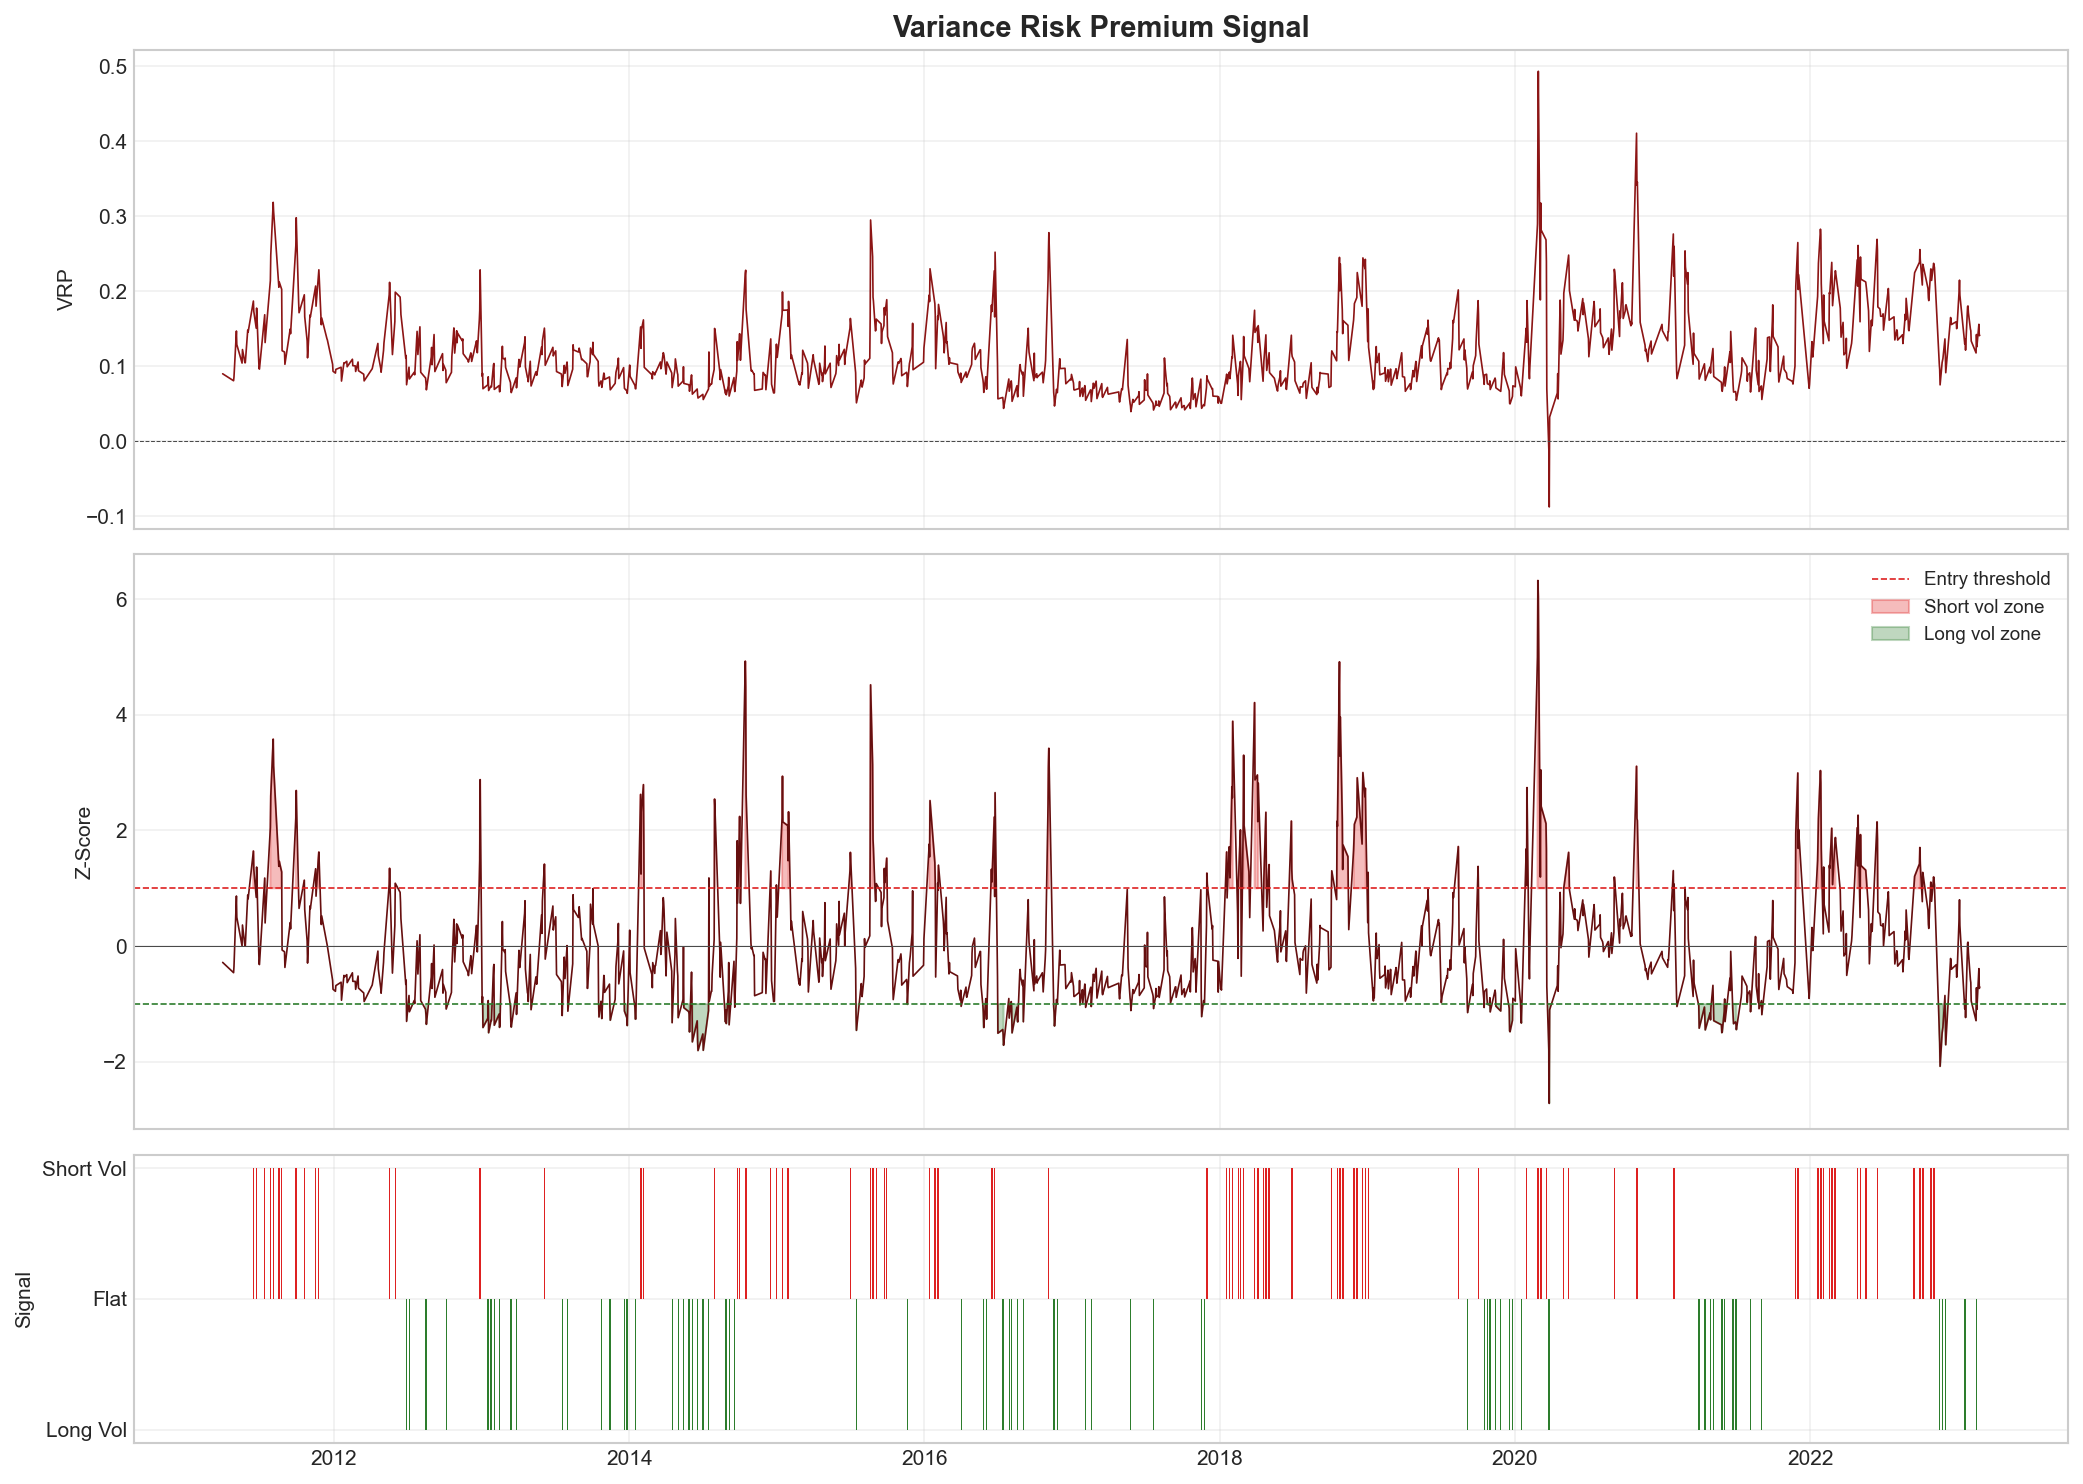
\includegraphics[width=\textwidth]{05_vrp_signal.png}
    \caption{VRP signal z-score and discrete trading signals over time.}
\end{figure}

\begin{figure}[H]
    \centering
    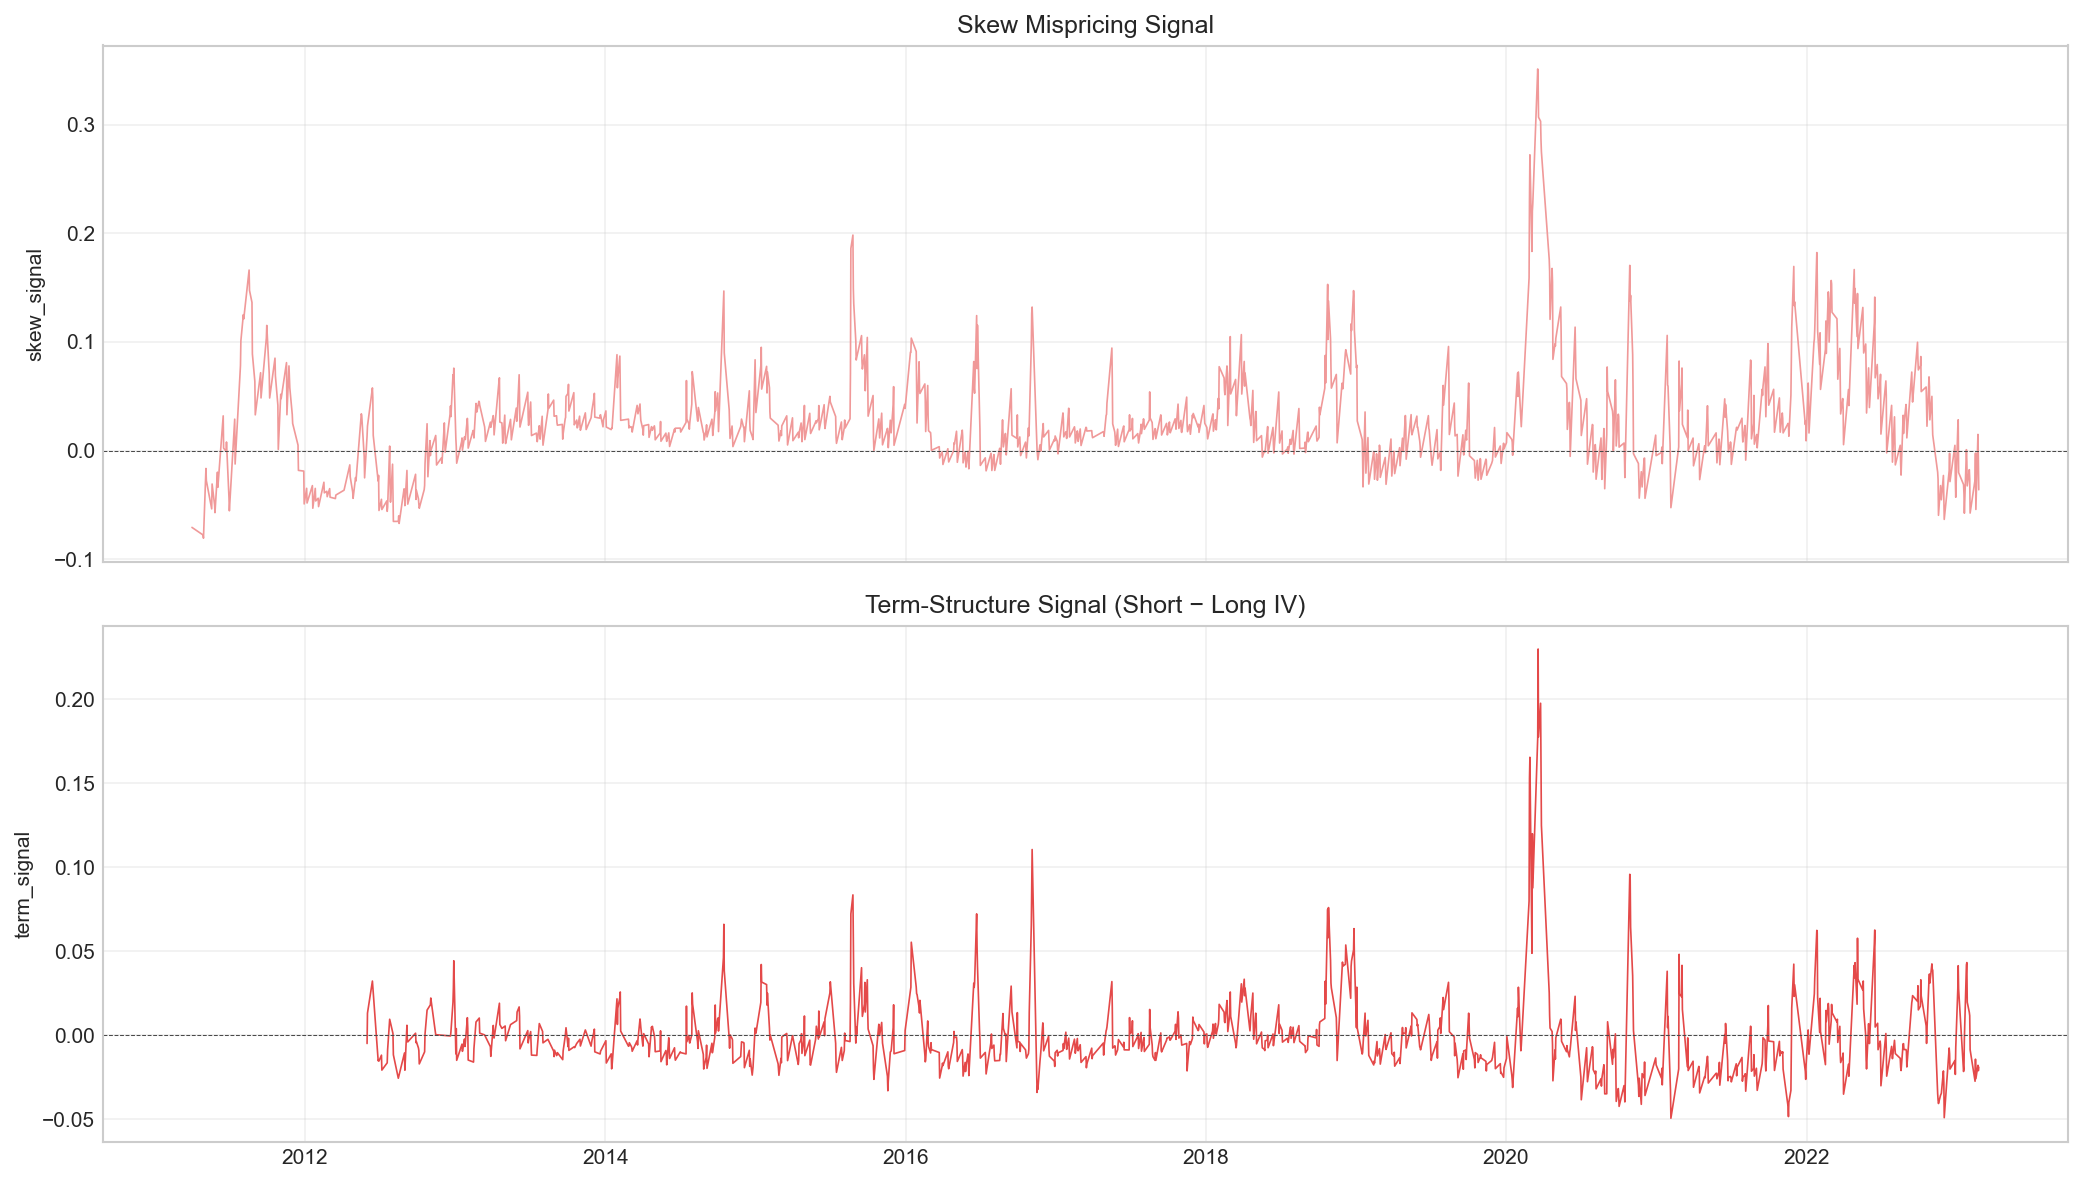
\includegraphics[width=\textwidth]{06_surface_signals.png}
    \caption{Skew and term-structure surface signals.}
\end{figure}

\begin{figure}[H]
    \centering
    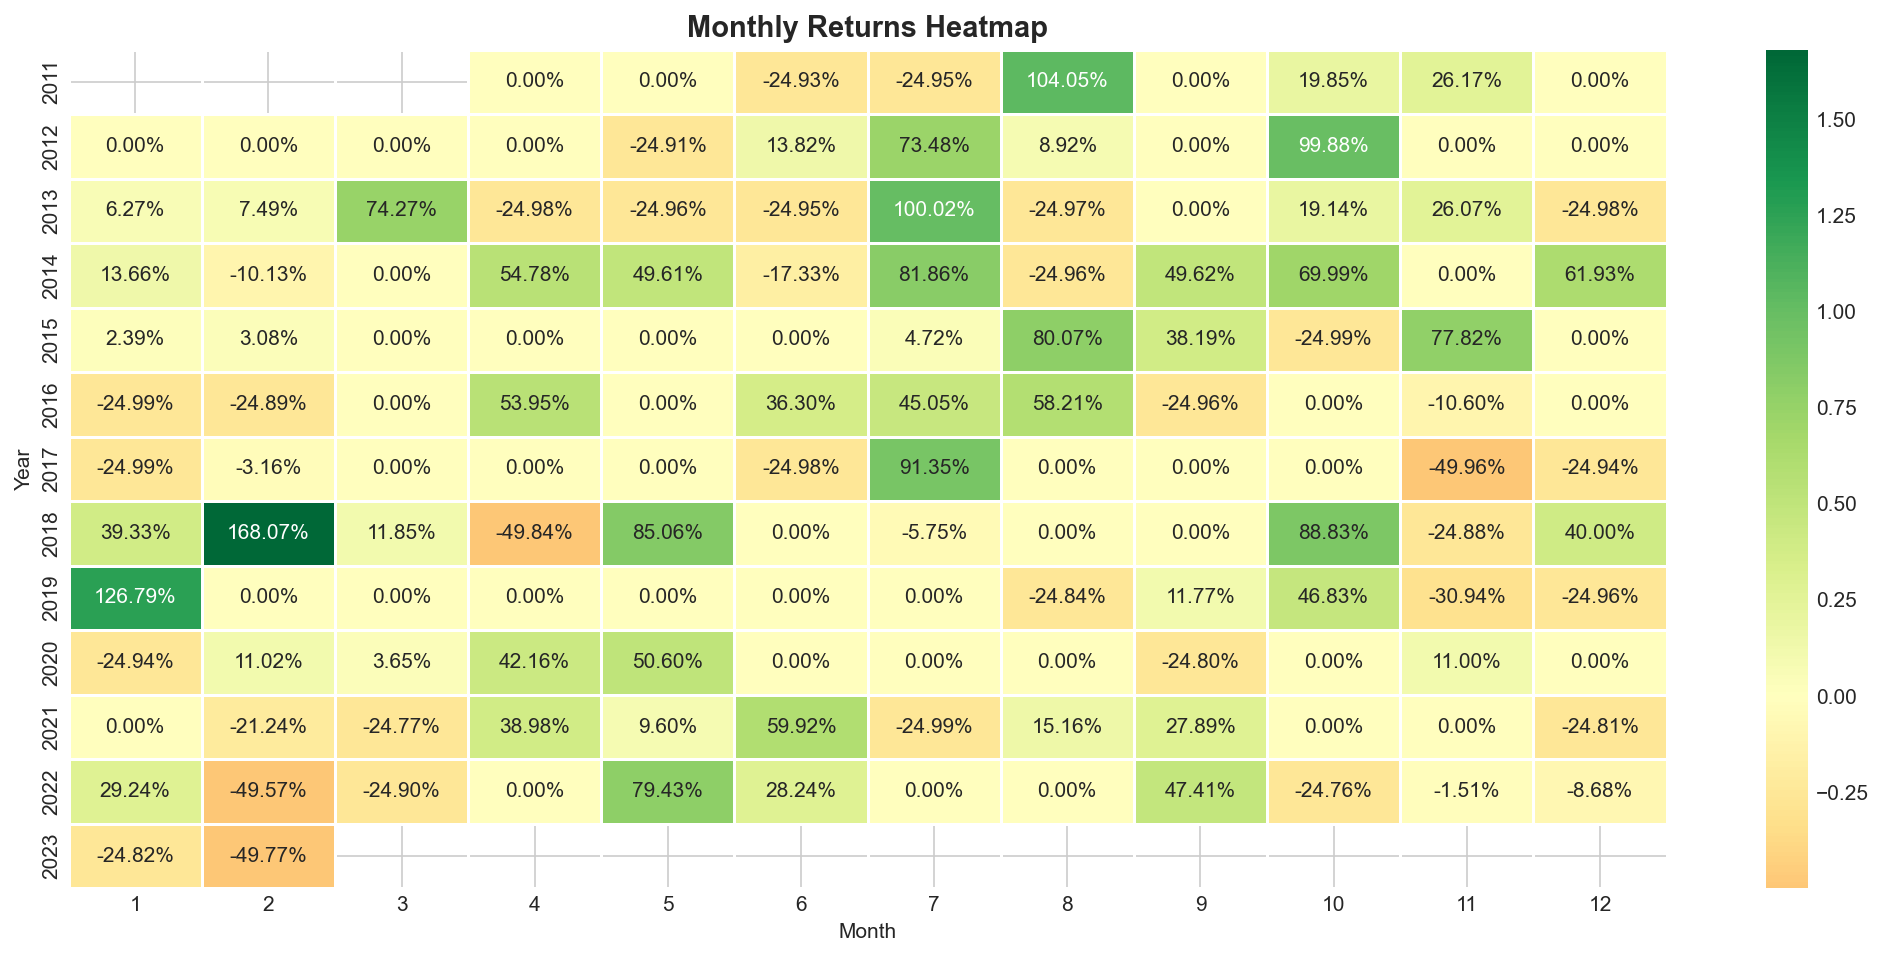
\includegraphics[width=\textwidth]{09_monthly_returns.png}
    \caption{Monthly return heatmap.}
\end{figure}

\begin{figure}[H]
    \centering
    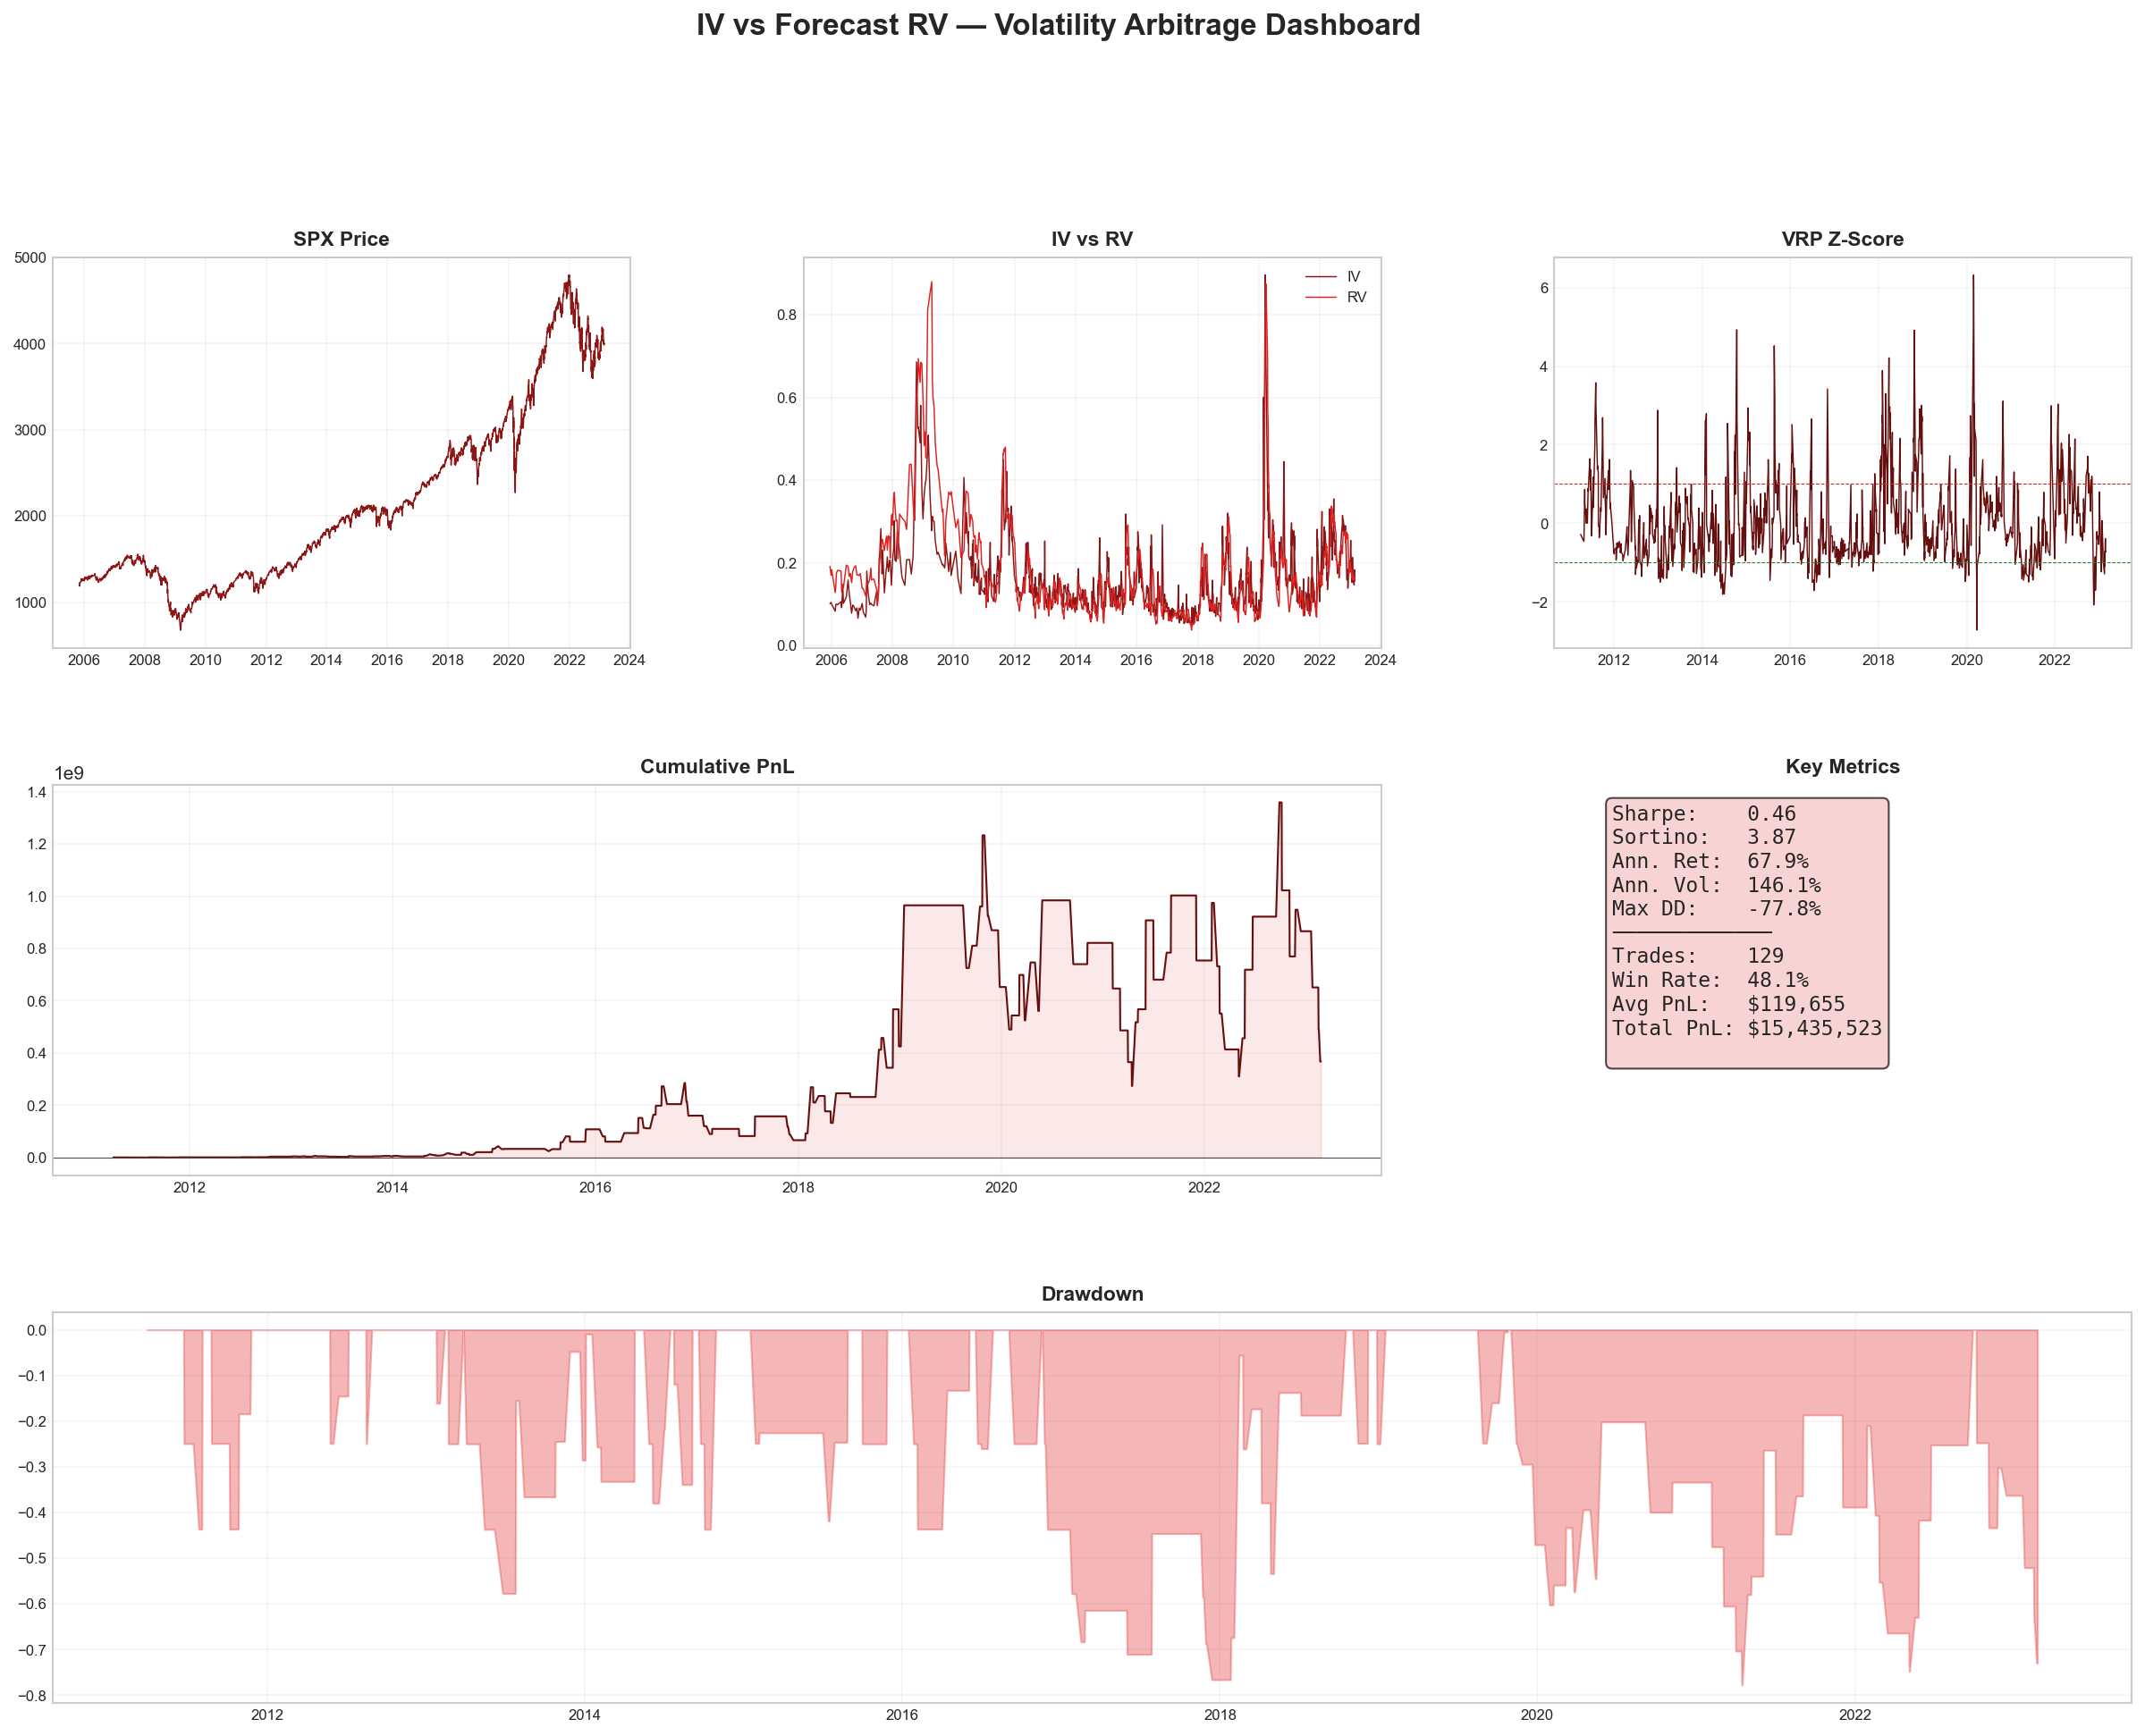
\includegraphics[width=\textwidth]{12_summary_dashboard.png}
    \caption{Summary performance dashboard.}
\end{figure}

\end{document}
